% Options for packages loaded elsewhere
\PassOptionsToPackage{unicode}{hyperref}
\PassOptionsToPackage{hyphens}{url}
%
\documentclass[
]{article}
\usepackage{lmodern}
\usepackage{amssymb,amsmath}
\usepackage{ifxetex,ifluatex}
\ifnum 0\ifxetex 1\fi\ifluatex 1\fi=0 % if pdftex
  \usepackage[T1]{fontenc}
  \usepackage[utf8]{inputenc}
  \usepackage{textcomp} % provide euro and other symbols
\else % if luatex or xetex
  \usepackage{unicode-math}
  \defaultfontfeatures{Scale=MatchLowercase}
  \defaultfontfeatures[\rmfamily]{Ligatures=TeX,Scale=1}
\fi
% Use upquote if available, for straight quotes in verbatim environments
\IfFileExists{upquote.sty}{\usepackage{upquote}}{}
\IfFileExists{microtype.sty}{% use microtype if available
  \usepackage[]{microtype}
  \UseMicrotypeSet[protrusion]{basicmath} % disable protrusion for tt fonts
}{}
\makeatletter
\@ifundefined{KOMAClassName}{% if non-KOMA class
  \IfFileExists{parskip.sty}{%
    \usepackage{parskip}
  }{% else
    \setlength{\parindent}{0pt}
    \setlength{\parskip}{6pt plus 2pt minus 1pt}}
}{% if KOMA class
  \KOMAoptions{parskip=half}}
\makeatother
\usepackage{xcolor}
\IfFileExists{xurl.sty}{\usepackage{xurl}}{} % add URL line breaks if available
\IfFileExists{bookmark.sty}{\usepackage{bookmark}}{\usepackage{hyperref}}
\hypersetup{
  hidelinks,
  pdfcreator={LaTeX via pandoc}}
\urlstyle{same} % disable monospaced font for URLs
\usepackage[margin=1in]{geometry}
\usepackage{graphicx,grffile}
\makeatletter
\def\maxwidth{\ifdim\Gin@nat@width>\linewidth\linewidth\else\Gin@nat@width\fi}
\def\maxheight{\ifdim\Gin@nat@height>\textheight\textheight\else\Gin@nat@height\fi}
\makeatother
% Scale images if necessary, so that they will not overflow the page
% margins by default, and it is still possible to overwrite the defaults
% using explicit options in \includegraphics[width, height, ...]{}
\setkeys{Gin}{width=\maxwidth,height=\maxheight,keepaspectratio}
% Set default figure placement to htbp
\makeatletter
\def\fps@figure{htbp}
\makeatother
\setlength{\emergencystretch}{3em} % prevent overfull lines
\providecommand{\tightlist}{%
  \setlength{\itemsep}{0pt}\setlength{\parskip}{0pt}}
\setcounter{secnumdepth}{-\maxdimen} % remove section numbering
%latex header to wrap code lines in .pdf

\usepackage{fvextra}
\DefineVerbatimEnvironment{Highlighting}{Verbatim}{breaklines,commandchars=\\\{\}}

% To keep the figure from floating around
% All figures should be forced in-place via the [H]ERE float specification.
\usepackage{float}
\floatplacement{figure}{H}
%\floatplacement{figure}{!htbp}

\date{}

\begin{document}

\hypertarget{report-of-the-fit}{%
\section{Report of the fit}\label{report-of-the-fit}}

\hypertarget{fit-summary}{%
\subsection{Fit summary}\label{fit-summary}}

Description: PV19 version x, parameters for NNLL. Trying the parameters
that gave chi2 = 1.65708 for replica 0 when minimised with ceres. Minuit
with the same parameters, starting from the same fitcofig, didn't
converge.\\
Minimiser: ceres\\
Random seed: 1234\\
Maximum values allowed for \(q_T / Q\): 0.2\\
Cut on the error function: 4\\
Parameterisation: PV19x\\
Initial parameters fluctuations: True\\
Explicit formula:

\[f_{\rm NP}(x,\zeta, b_T)= \Biggl(
\frac{1-\lambda}{1 + g_1(x) b_T^2/4} + \lambda \exp \left(-g_{1B}(x) b_T^2 / 4 \right)\Biggr) \exp\left[- g_2 \log\left(\frac{\zeta}{Q_0^2}\right) b_T^2/4 - g_{2B} \log\left(\frac{\zeta}{Q_0^2}\right) b_T^4/4 \right]\]\[g_1(x) = \frac{N_1}{x\sigma} \exp\left[ - \frac{\ln^2\left(\frac{x}{\alpha}\right)}{2 \sigma^2} \right]\]\[g_{1B}(x) = \frac{N_{1B}}{x\sigma_B} \exp\left[ - \frac{\ln^2\left(\frac{x}{\alpha_B}\right)}{2 \sigma_B^2} \right]\]\[Q_0^2 = 1\;{\rm GeV}^2\]
\(t_0\) prescription: True

\begin{table}[h]

\centering

\begin{tabular}{|c|c|c|c|c|c|c|c|c|} \hline

\textbf{\(g_2\)} & \textbf{\(N_1\)} & \textbf{\(\alpha\)} & \textbf{\(\sigma\)} & \textbf{\(\lambda\)} & \textbf{\(N_{1B}\)} & \textbf{\(\alpha_B\)} & \textbf{\(\sigma_B\)} & \textbf{\(g_{2B}\)} \\ \hline

0.005144 & 0.68535248 & 0.21943481 & 0.3329461 & 0.66627605 & 0.0387879 & 0.075758463 & 0.34845635 & 0.019224141 \\ \hline

\end{tabular}

\caption{}

\end{table}

\hypertarget{theory-summary}{%
\subsection{Theory summary}\label{theory-summary}}

Collinear PDF set: MMHT2014nlo68cl member 0\\
Collinear FF set: DSS14\_NLO\_PiSum member 0\\
\(b^*\) prescription: bstarmin\\
Perturbative order: NNLL\\
Reference value of the fine-structure constant:
\(\alpha(Q = 91.1876\;{\rm GeV}) = 0.00776578395589\) (running True)

\hypertarget{global-statistical-estimators}{%
\subsection{Global statistical
estimators}\label{global-statistical-estimators}}

\(N_{rep}\) = 270\\
\(\chi_{0}^2\) = 1.6571\\
\(\chi_{mean}^2\) = 1.6392\\
\(\langle\chi^2\rangle \pm \sigma_{\chi^2}\) = 1.7007 \(\pm\) 0.0802\\
\(\langle E \rangle \pm \sigma_{E}\) = 2.6694 \(\pm\) 0.2184

\hypertarget{parameters}{%
\subsection{Parameters}\label{parameters}}

\begin{table}[h]

\centering

\begin{tabular}{|c|c|c|c|} \hline

\textbf{Parameter} & \textbf{Central replica} & \textbf{Average over
replicas} & \textbf{Fixed} \\ \hline

\(g_2\) & -0.09141059 & -0.07295757 \(\pm\) 0.02515211 & False \\ \hline
\(N_1\) & 5.3603904 & 12.69051436 \(\pm\) 47.81474706 & False \\ \hline
\(\alpha\) & 1.0686624 & 2.06976511 \(\pm\) 5.84855393 & False \\ \hline
\(\sigma\) & 0.93749188 & 0.8379623 \(\pm\) 0.29305058 & False \\ \hline
\(\lambda\) & 0.49349918 & 0.51210077 \(\pm\)
0.09098696 & False \\ \hline
\(N_{1B}\) & 0.040693304 & 0.04323806 \(\pm\)
0.29300377 & False \\ \hline
\(\alpha_B\) & 0.052748277 & 0.29790959 \(\pm\)
1.30094204 & False \\ \hline
\(\sigma_B\) & 0.56928194 & 1.05628826 \(\pm\)
21.49245902 & False \\ \hline
\(g_{2B}\) & 0.034354286 & 0.03183429 \(\pm\)
0.01009458 & False \\ \hline

\end{tabular}

\caption{}

\end{table}

\begin{figure}
\centering
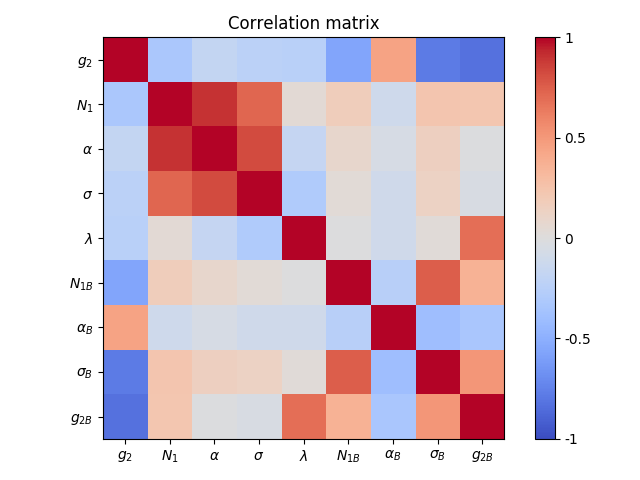
\includegraphics{pngplots/CorrelationMatrix.png}
\caption{Fitted parameter correlation matrix}
\end{figure}

\hypertarget{fit-properties}{%
\subsection{Fit properties}\label{fit-properties}}

\begin{figure}
\centering
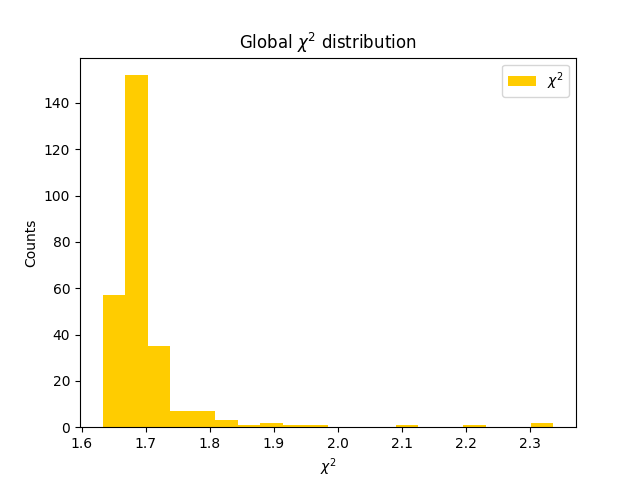
\includegraphics{pngplots/Globalchi2.png}
\caption{Global \(\chi^2\) distribution}
\end{figure}

\begin{figure}
\centering
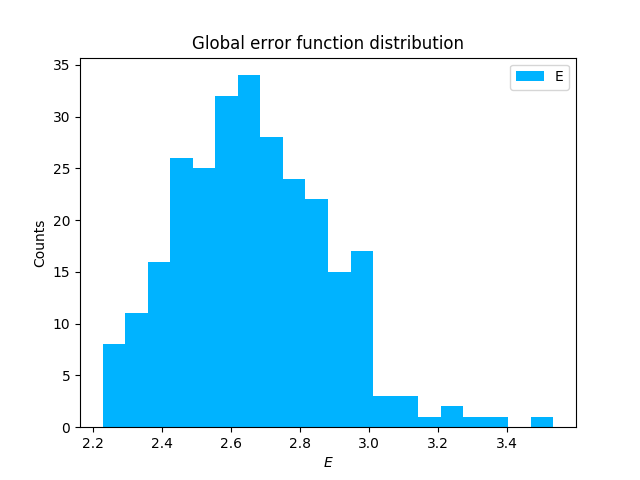
\includegraphics{pngplots/GlobalErrorFunction.png}
\caption{Global error function distribution}
\end{figure}

\begin{figure}
\centering
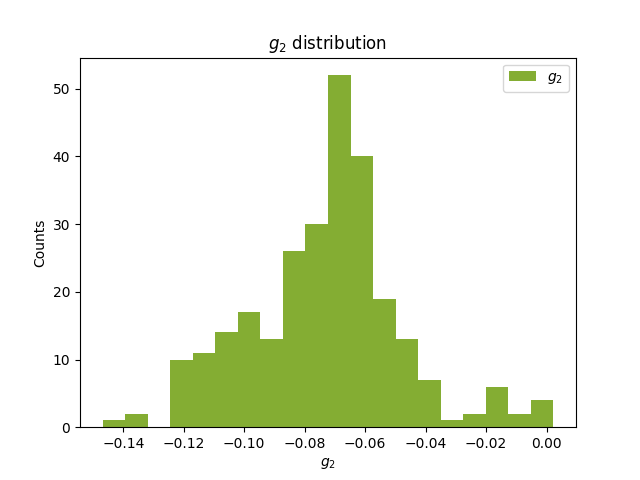
\includegraphics{pngplots/param0.png}
\caption{\(g_2\) distribution}
\end{figure}

\begin{figure}
\centering
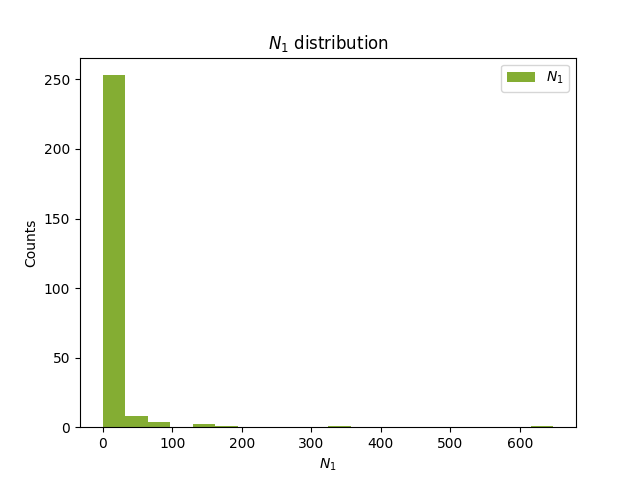
\includegraphics{pngplots/param1.png}
\caption{\(N_1\) distribution}
\end{figure}

\begin{figure}
\centering
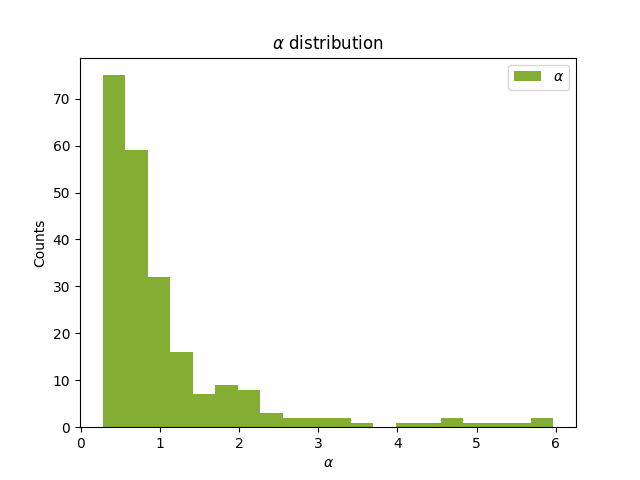
\includegraphics{pngplots/param2.png}
\caption{\(\alpha\) distribution}
\end{figure}

\begin{figure}
\centering
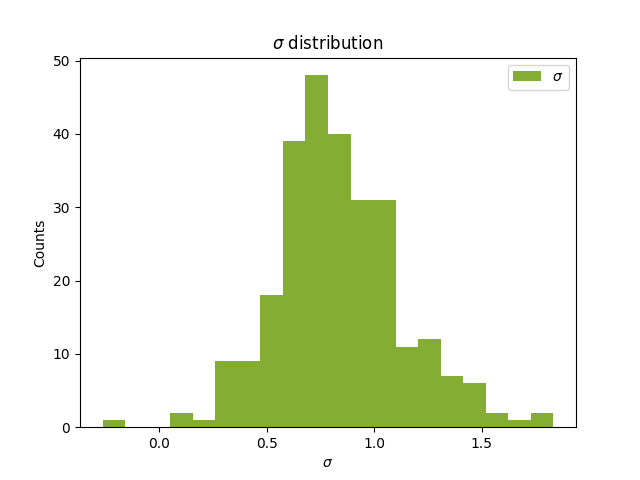
\includegraphics{pngplots/param3.png}
\caption{\(\sigma\) distribution}
\end{figure}

\begin{figure}
\centering
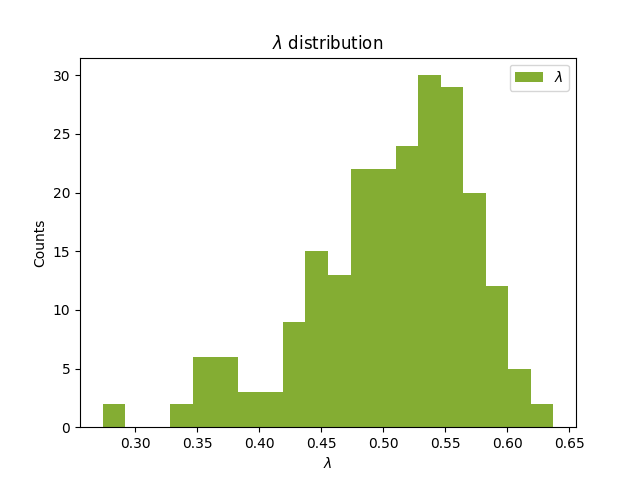
\includegraphics{pngplots/param4.png}
\caption{\(\lambda\) distribution}
\end{figure}

\begin{figure}
\centering
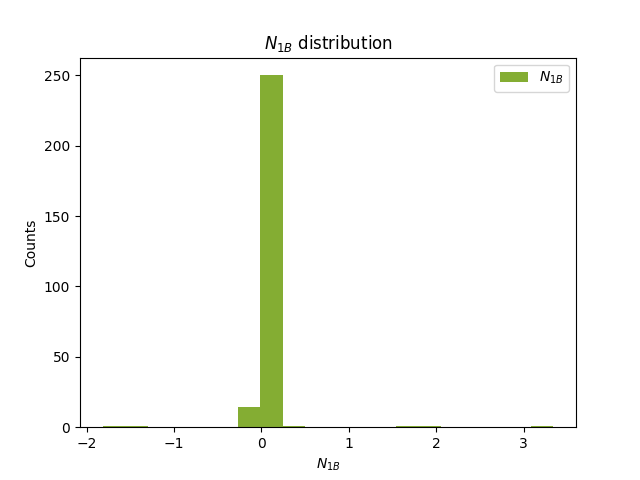
\includegraphics{pngplots/param5.png}
\caption{\(N_{1B}\) distribution}
\end{figure}

\begin{figure}
\centering
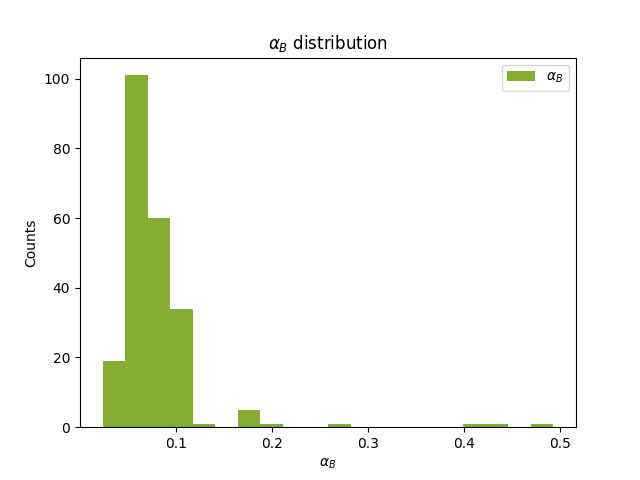
\includegraphics{pngplots/param6.png}
\caption{\(\alpha_B\) distribution}
\end{figure}

\begin{figure}
\centering
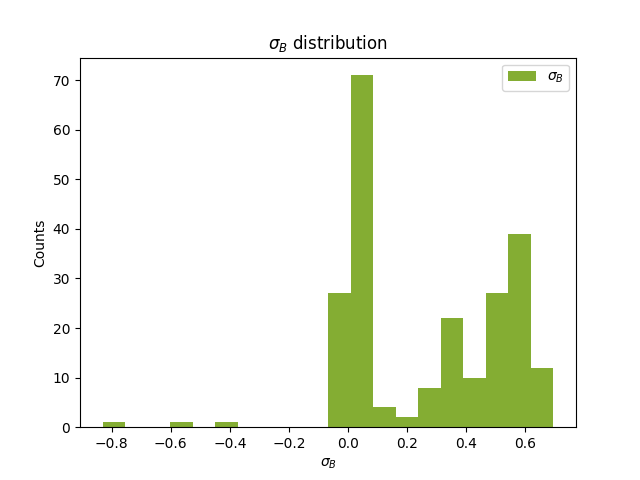
\includegraphics{pngplots/param7.png}
\caption{\(\sigma_B\) distribution}
\end{figure}

\begin{figure}
\centering
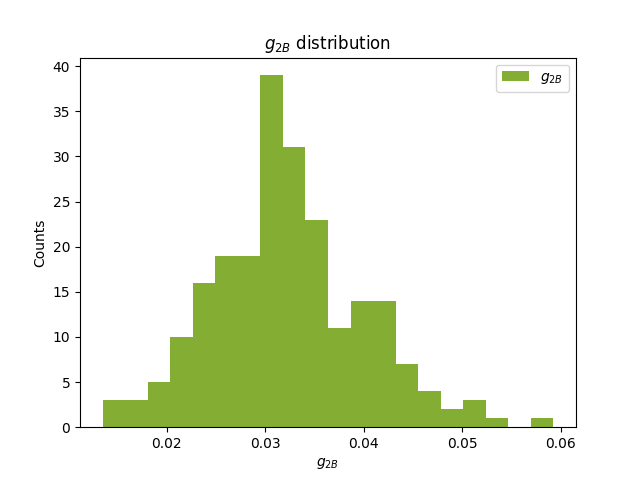
\includegraphics{pngplots/param8.png}
\caption{\(g_{2B}\) distribution}
\end{figure}

\hypertarget{table-of-chi2s}{%
\subsection{\texorpdfstring{Table of
\(\chi^2\)'s}{Table of \textbackslash chi\^{}2's}}\label{table-of-chi2s}}

\begin{table}[h]

\centering

\begin{tabular}{|c|c|c|c|c|} \hline

\textbf{Experiment} & \textbf{Number of
points} & \textbf{\(\chi_{D}^2\)} & \textbf{\(\chi_{\lambda}^2\)} & \textbf{\(\chi^2\)} \\ \hline

E605\_Q\_7\_8 & 7 & 0.4814 & 0.0307 & 0.5121 \\ \hline
E605\_Q\_8\_9 & 8 & 0.9948 & 0.0176 & 1.0124 \\ \hline
E605\_Q\_10.5\_11.5 & 10 & 0.494 & 0.1396 & 0.6336 \\ \hline
E288\_200\_Q\_4\_5 & 4 & 0.9291 & 0.8595 & 1.7885 \\ \hline
E288\_200\_Q\_5\_6 & 5 & 2.3107 & 0.3547 & 2.6654 \\ \hline
E288\_200\_Q\_6\_7 & 6 & 0.7947 & 0.2112 & 1.0059 \\ \hline
E288\_200\_Q\_7\_8 & 7 & 0.9887 & 0.032 & 1.0206 \\ \hline
E288\_200\_Q\_8\_9 & 8 & 0.7359 & 0.0059 & 0.7419 \\ \hline
E288\_300\_Q\_4\_5 & 4 & 0.7784 & 0.3426 & 1.121 \\ \hline
E288\_300\_Q\_5\_6 & 5 & 1.3997 & 0.1 & 1.4997 \\ \hline
E288\_300\_Q\_6\_7 & 6 & 1.042 & 0.0398 & 1.0818 \\ \hline
E288\_300\_Q\_7\_8 & 7 & 0.3439 & 0.0425 & 0.3864 \\ \hline
E288\_300\_Q\_8\_9 & 8 & 0.3919 & 0.0384 & 0.4303 \\ \hline
E288\_400\_Q\_5\_6 & 5 & 0.9446 & 0.001 & 0.9456 \\ \hline
E288\_400\_Q\_6\_7 & 6 & 0.5281 & 0.0068 & 0.5349 \\ \hline
E288\_400\_Q\_7\_8 & 7 & 0.2499 & 0.0139 & 0.2637 \\ \hline
E288\_400\_Q\_8\_9 & 8 & 0.5613 & 0.0126 & 0.574 \\ \hline
E288\_400\_Q\_11\_12 & 11 & 0.5749 & 0.0068 & 0.5817 \\ \hline
E288\_400\_Q\_12\_13 & 12 & 0.5394 & 0.0113 & 0.5507 \\ \hline
E288\_400\_Q\_13\_14 & 12 & 0.3455 & 0.0363 & 0.3817 \\ \hline
STAR\_510 & 7 & 1.192 & 0.0136 & 1.2056 \\ \hline
CDF\_RunI & 25 & 0.6522 & 0.1484 & 0.8006 \\ \hline
CDF\_RunII & 26 & 1.2759 & 0.0074 & 1.2833 \\ \hline
D0\_RunI & 12 & 0.6652 & 0.0018 & 0.667 \\ \hline
D0\_RunII & 5 & 0.9114 & 0.2907 & 1.2022 \\ \hline
D0\_RunIImu & 3 & 0.1197 & 0.0844 & 0.2041 \\ \hline
LHCb\_7TeV & 7 & 1.945 & 0.8427 & 2.7877 \\ \hline
LHCb\_8TeV & 7 & 1.9245 & 1.453 & 3.3775 \\ \hline
LHCb\_13TeV & 7 & 1.4927 & 0.2893 & 1.782 \\ \hline
CMS\_7TeV & 4 & 2.8928 & 0 & 2.8928 \\ \hline
CMS\_8TeV & 4 & 1.4845 & 0.1782 & 1.6627 \\ \hline
ATLAS\_7TeV\_y\_0\_1 & 6 & 6.9545 & 1.0911 & 8.0455 \\ \hline
ATLAS\_7TeV\_y\_1\_2 & 6 & 4.9261 & 0.4825 & 5.4086 \\ \hline
ATLAS\_7TeV\_y\_2\_2.4 & 6 & 1.8076 & 0.0099 & 1.8176 \\ \hline
ATLAS\_8TeV\_y\_0\_0.4 & 6 & 4.7783 & 0.9776 & 5.756 \\ \hline
ATLAS\_8TeV\_y\_0.4\_0.8 & 6 & 6.6974 & 1.5469 & 8.2443 \\ \hline
ATLAS\_8TeV\_y\_0.8\_1.2 & 6 & 4.3581 & 0.6689 & 5.027 \\ \hline
ATLAS\_8TeV\_y\_1.2\_1.6 & 6 & 2.9433 & 0.4249 & 3.3682 \\ \hline
ATLAS\_8TeV\_y\_1.6\_2 & 6 & 2.5563 & 0.2696 & 2.8259 \\ \hline
ATLAS\_8TeV\_y\_2\_2.4 & 6 & 1.2834 & 0.1619 & 1.4453 \\ \hline
ATLAS\_8TeV\_Q\_46\_66 & 4 & 0.7685 & 0.0368 & 0.8053 \\ \hline
ATLAS\_8TeV\_Q\_116\_150 & 8 & 1.1501 & 0.0073 & 1.1574 \\ \hline
Total & 319 & - & - & 1.6571 \\ \hline

\end{tabular}

\caption{Central-replica \(\chi^2\)'s:}

\end{table}

\begin{table}[h]

\centering

\begin{tabular}{|c|c|c|c|c|} \hline

\textbf{Experiment} & \textbf{Number of
points} & \textbf{\(\chi_{D}^2\)} & \textbf{\(\chi_{\lambda}^2\)} & \textbf{\(\chi^2\)} \\ \hline

E605\_Q\_7\_8 & 7 & 0.632 & 0.0898 & 0.7218 \\ \hline
E605\_Q\_8\_9 & 8 & 1.2311 & 0.048 & 1.2791 \\ \hline
E605\_Q\_10.5\_11.5 & 10 & 0.3645 & 0.1015 & 0.466 \\ \hline
E288\_200\_Q\_4\_5 & 4 & 0.4534 & 0.4421 & 0.8956 \\ \hline
E288\_200\_Q\_5\_6 & 5 & 1.3314 & 0.2707 & 1.6021 \\ \hline
E288\_200\_Q\_6\_7 & 6 & 0.5796 & 0.1765 & 0.7562 \\ \hline
E288\_200\_Q\_7\_8 & 7 & 0.9051 & 0.0334 & 0.9385 \\ \hline
E288\_200\_Q\_8\_9 & 8 & 0.9342 & 0.0128 & 0.9469 \\ \hline
E288\_300\_Q\_4\_5 & 4 & 0.5336 & 0.16 & 0.6935 \\ \hline
E288\_300\_Q\_5\_6 & 5 & 1.1461 & 0.0595 & 1.2056 \\ \hline
E288\_300\_Q\_6\_7 & 6 & 0.9439 & 0.0265 & 0.9704 \\ \hline
E288\_300\_Q\_7\_8 & 7 & 0.326 & 0.033 & 0.359 \\ \hline
E288\_300\_Q\_8\_9 & 8 & 0.2817 & 0.0393 & 0.321 \\ \hline
E288\_400\_Q\_5\_6 & 5 & 1.0811 & 0.0171 & 1.0982 \\ \hline
E288\_400\_Q\_6\_7 & 6 & 0.6129 & 0.0299 & 0.6427 \\ \hline
E288\_400\_Q\_7\_8 & 7 & 0.2957 & 0.0462 & 0.3419 \\ \hline
E288\_400\_Q\_8\_9 & 8 & 0.7447 & 0.0408 & 0.7856 \\ \hline
E288\_400\_Q\_11\_12 & 11 & 0.839 & 0.0141 & 0.8531 \\ \hline
E288\_400\_Q\_12\_13 & 12 & 0.8667 & 0.0173 & 0.884 \\ \hline
E288\_400\_Q\_13\_14 & 12 & 0.8895 & 0.066 & 0.9555 \\ \hline
STAR\_510 & 7 & 1.1469 & 0.0372 & 1.1841 \\ \hline
CDF\_RunI & 25 & 0.5739 & 0.1421 & 0.716 \\ \hline
CDF\_RunII & 26 & 1.2356 & 0.006 & 1.2416 \\ \hline
D0\_RunI & 12 & 0.6384 & 0.0007 & 0.6391 \\ \hline
D0\_RunII & 5 & 1.0845 & 0.2943 & 1.3788 \\ \hline
D0\_RunIImu & 3 & 0.022 & 0.0333 & 0.0554 \\ \hline
LHCb\_7TeV & 7 & 1.682 & 0.8471 & 2.5291 \\ \hline
LHCb\_8TeV & 7 & 1.8199 & 1.3821 & 3.202 \\ \hline
LHCb\_13TeV & 7 & 1.3368 & 0.2691 & 1.6059 \\ \hline
CMS\_7TeV & 4 & 2.8768 & 0 & 2.8768 \\ \hline
CMS\_8TeV & 4 & 1.5098 & 0.1835 & 1.6933 \\ \hline
ATLAS\_7TeV\_y\_0\_1 & 6 & 6.9378 & 1.0929 & 8.0307 \\ \hline
ATLAS\_7TeV\_y\_1\_2 & 6 & 4.8183 & 0.4907 & 5.3091 \\ \hline
ATLAS\_7TeV\_y\_2\_2.4 & 6 & 1.6825 & 0.01 & 1.6924 \\ \hline
ATLAS\_8TeV\_y\_0\_0.4 & 6 & 4.7797 & 1.0131 & 5.7928 \\ \hline
ATLAS\_8TeV\_y\_0.4\_0.8 & 6 & 6.5292 & 1.5932 & 8.1224 \\ \hline
ATLAS\_8TeV\_y\_0.8\_1.2 & 6 & 4.3571 & 0.6881 & 5.0452 \\ \hline
ATLAS\_8TeV\_y\_1.2\_1.6 & 6 & 2.9724 & 0.4409 & 3.4133 \\ \hline
ATLAS\_8TeV\_y\_1.6\_2 & 6 & 2.4292 & 0.2746 & 2.7039 \\ \hline
ATLAS\_8TeV\_y\_2\_2.4 & 6 & 1.1482 & 0.1534 & 1.3016 \\ \hline
ATLAS\_8TeV\_Q\_46\_66 & 4 & 0.716 & 0.0522 & 0.7682 \\ \hline
ATLAS\_8TeV\_Q\_116\_150 & 8 & 1.1316 & 0.0063 & 1.1379 \\ \hline
Total & 319 & - & - & 1.6392 \\ \hline

\end{tabular}

\caption{Mean-replica \(\chi^2\)'s:}

\end{table}

\begin{table}[h]

\centering

\begin{tabular}{|c|c|c|c|c|} \hline

\textbf{Experiment} & \textbf{Number of
points} & \textbf{\(\chi_{D}^2\)} & \textbf{\(\chi_{\lambda}^2\)} & \textbf{\(\chi^2\)} \\ \hline

E605\_Q\_7\_8 & 7 & 0.4513 \(\pm\) 0.2372 & 0.1896 \(\pm\)
0.3088 & 0.6409 \(\pm\) 0.2801 \\ \hline
E605\_Q\_8\_9 & 8 & 1.0562 \(\pm\) 0.2814 & 0.1272 \(\pm\)
0.1971 & 1.1835 \(\pm\) 0.3074 \\ \hline
E605\_Q\_10.5\_11.5 & 10 & 0.4632 \(\pm\) 0.2561 & 0.1994 \(\pm\)
0.2873 & 0.6626 \(\pm\) 0.2126 \\ \hline
E288\_200\_Q\_4\_5 & 4 & 0.5274 \(\pm\) 1.2228 & 1.1102 \(\pm\)
1.211 & 1.6376 \(\pm\) 0.4142 \\ \hline
E288\_200\_Q\_5\_6 & 5 & 2.0643 \(\pm\) 0.6861 & 0.4911 \(\pm\)
0.6232 & 2.5554 \(\pm\) 0.35 \\ \hline
E288\_200\_Q\_6\_7 & 6 & 0.6389 \(\pm\) 0.4078 & 0.3042 \(\pm\)
0.3518 & 0.9431 \(\pm\) 0.2271 \\ \hline
E288\_200\_Q\_7\_8 & 7 & 0.8732 \(\pm\) 0.2666 & 0.1173 \(\pm\)
0.1617 & 0.9905 \(\pm\) 0.2335 \\ \hline
E288\_200\_Q\_8\_9 & 8 & 0.6884 \(\pm\) 0.1436 & 0.0814 \(\pm\)
0.1216 & 0.7698 \(\pm\) 0.1338 \\ \hline
E288\_300\_Q\_4\_5 & 4 & 0.4581 \(\pm\) 0.7823 & 0.5634 \(\pm\)
0.7213 & 1.0215 \(\pm\) 0.2611 \\ \hline
E288\_300\_Q\_5\_6 & 5 & 1.1437 \(\pm\) 0.4287 & 0.2822 \(\pm\)
0.3808 & 1.4259 \(\pm\) 0.3134 \\ \hline
E288\_300\_Q\_6\_7 & 6 & 0.8482 \(\pm\) 0.365 & 0.1702 \(\pm\)
0.2521 & 1.0184 \(\pm\) 0.3057 \\ \hline
E288\_300\_Q\_7\_8 & 7 & 0.2174 \(\pm\) 0.2377 & 0.1527 \(\pm\)
0.2259 & 0.3701 \(\pm\) 0.1712 \\ \hline
E288\_300\_Q\_8\_9 & 8 & 0.3347 \(\pm\) 0.1636 & 0.1135 \(\pm\)
0.1742 & 0.4481 \(\pm\) 0.0798 \\ \hline
E288\_400\_Q\_5\_6 & 5 & 0.7207 \(\pm\) 0.4038 & 0.1706 \(\pm\)
0.2432 & 0.8913 \(\pm\) 0.3673 \\ \hline
E288\_400\_Q\_6\_7 & 6 & 0.4046 \(\pm\) 0.3472 & 0.1178 \(\pm\)
0.1577 & 0.5224 \(\pm\) 0.3521 \\ \hline
E288\_400\_Q\_7\_8 & 7 & 0.1702 \(\pm\) 0.2897 & 0.1243 \(\pm\)
0.1923 & 0.2944 \(\pm\) 0.2781 \\ \hline
E288\_400\_Q\_8\_9 & 8 & 0.524 \(\pm\) 0.1912 & 0.0937 \(\pm\)
0.1567 & 0.6176 \(\pm\) 0.1931 \\ \hline
E288\_400\_Q\_11\_12 & 11 & 0.5413 \(\pm\) 0.1319 & 0.0481 \(\pm\)
0.0671 & 0.5894 \(\pm\) 0.136 \\ \hline
E288\_400\_Q\_12\_13 & 12 & 0.5298 \(\pm\) 0.0984 & 0.0549 \(\pm\)
0.0748 & 0.5847 \(\pm\) 0.1012 \\ \hline
E288\_400\_Q\_13\_14 & 12 & 0.3521 \(\pm\) 0.1254 & 0.0806 \(\pm\)
0.0861 & 0.4327 \(\pm\) 0.1506 \\ \hline
STAR\_510 & 7 & 1.0753 \(\pm\) 0.2297 & 0.1179 \(\pm\) 0.1801 & 1.1932
\(\pm\) 0.1511 \\ \hline
CDF\_RunI & 25 & 0.6244 \(\pm\) 0.1758 & 0.1993 \(\pm\) 0.1712 & 0.8238
\(\pm\) 0.0478 \\ \hline
CDF\_RunII & 26 & 1.2861 \(\pm\) 0.2307 & 0.0594 \(\pm\) 0.0772 & 1.3455
\(\pm\) 0.2215 \\ \hline
D0\_RunI & 12 & 0.628 \(\pm\) 0.1273 & 0.0682 \(\pm\) 0.0998 & 0.6961
\(\pm\) 0.0743 \\ \hline
D0\_RunII & 5 & 0.6847 \(\pm\) 0.6844 & 0.4929 \(\pm\) 0.5676 & 1.1776
\(\pm\) 0.3549 \\ \hline
D0\_RunIImu & 3 & -0.3655 \(\pm\) 0.6009 & 0.5434 \(\pm\)
0.5577 & 0.1778 \(\pm\) 0.2622 \\ \hline
LHCb\_7TeV & 7 & 1.7619 \(\pm\) 0.7676 & 1.068 \(\pm\) 0.7369 & 2.8299
\(\pm\) 0.194 \\ \hline
LHCb\_8TeV & 7 & 1.9023 \(\pm\) 0.9789 & 1.5711 \(\pm\) 0.9045 & 3.4734
\(\pm\) 0.3695 \\ \hline
LHCb\_13TeV & 7 & 1.4037 \(\pm\) 0.4286 & 0.3604 \(\pm\) 0.4047 & 1.7641
\(\pm\) 0.1 \\ \hline
CMS\_7TeV & 4 & 2.9071 \(\pm\) 0.056 & 0.0 \(\pm\) 0.0 & 2.9071 \(\pm\)
0.056 \\ \hline
CMS\_8TeV & 4 & 1.4376 \(\pm\) 0.2788 & 0.2545 \(\pm\) 0.2312 & 1.6921
\(\pm\) 0.1362 \\ \hline
ATLAS\_7TeV\_y\_0\_1 & 6 & 7.0564 \(\pm\) 0.9804 & 1.1916 \(\pm\)
0.5676 & 8.2479 \(\pm\) 0.7257 \\ \hline
ATLAS\_7TeV\_y\_1\_2 & 6 & 5.0049 \(\pm\) 0.4967 & 0.5612 \(\pm\)
0.3415 & 5.5662 \(\pm\) 0.3634 \\ \hline
ATLAS\_7TeV\_y\_2\_2.4 & 6 & 1.8566 \(\pm\) 0.1681 & 0.0263 \(\pm\)
0.0353 & 1.8829 \(\pm\) 0.1652 \\ \hline
ATLAS\_8TeV\_y\_0\_0.4 & 6 & 5.0304 \(\pm\) 0.7671 & 1.0682 \(\pm\)
0.5054 & 6.0986 \(\pm\) 0.6327 \\ \hline
ATLAS\_8TeV\_y\_0.4\_0.8 & 6 & 6.7856 \(\pm\) 0.7991 & 1.6653 \(\pm\)
0.7173 & 8.4509 \(\pm\) 0.4889 \\ \hline
ATLAS\_8TeV\_y\_0.8\_1.2 & 6 & 4.321 \(\pm\) 0.4412 & 0.6707 \(\pm\)
0.3289 & 4.9918 \(\pm\) 0.3395 \\ \hline
ATLAS\_8TeV\_y\_1.2\_1.6 & 6 & 2.9251 \(\pm\) 0.4087 & 0.4814 \(\pm\)
0.3273 & 3.4065 \(\pm\) 0.2666 \\ \hline
ATLAS\_8TeV\_y\_1.6\_2 & 6 & 2.6986 \(\pm\) 0.4661 & 0.3245 \(\pm\)
0.3115 & 3.0231 \(\pm\) 0.3412 \\ \hline
ATLAS\_8TeV\_y\_2\_2.4 & 6 & 1.5245 \(\pm\) 0.5671 & 0.2544 \(\pm\)
0.227 & 1.7789 \(\pm\) 0.5397 \\ \hline
ATLAS\_8TeV\_Q\_46\_66 & 4 & 0.6217 \(\pm\) 0.3154 & 0.2169 \(\pm\)
0.3072 & 0.8386 \(\pm\) 0.1187 \\ \hline
ATLAS\_8TeV\_Q\_116\_150 & 8 & 1.0732 \(\pm\) 0.1956 & 0.1106 \(\pm\)
0.1839 & 1.1838 \(\pm\) 0.067 \\ \hline
Total & 319 & - & - & 1.7007 \(\pm\) 0.0802 \\ \hline

\end{tabular}

\caption{Average-over-replicas \(\chi^2\)'s:}

\end{table}

\hypertarget{tmds-in-k_t-space}{%
\subsection{\texorpdfstring{TMDs in \(k_T\)
space}{TMDs in k\_T space}}\label{tmds-in-k_t-space}}

\begin{figure}
\centering
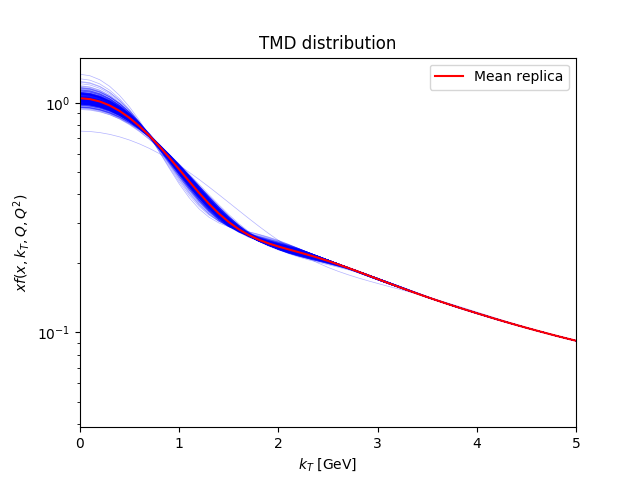
\includegraphics{pngplots/tmd_1_2_0.001.png}
\caption{TMD PDF of the \(d\) at \(Q = 2\) GeV and \(x = 0.001\)}
\end{figure}

\begin{figure}
\centering
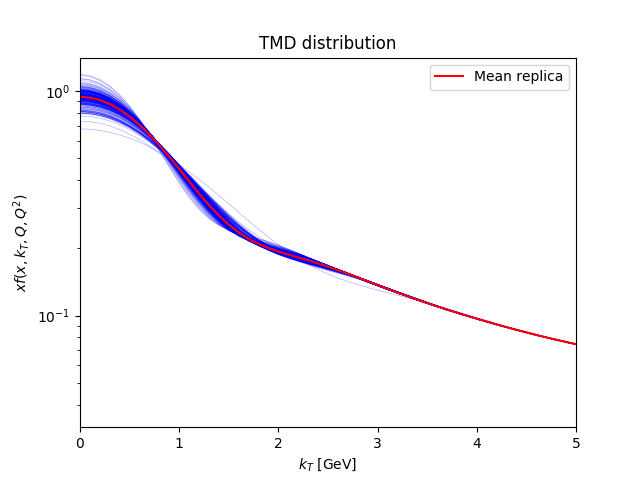
\includegraphics{pngplots/tmd_1_2_0.01.png}
\caption{TMD PDF of the \(d\) at \(Q = 2\) GeV and \(x = 0.01\)}
\end{figure}

\begin{figure}
\centering
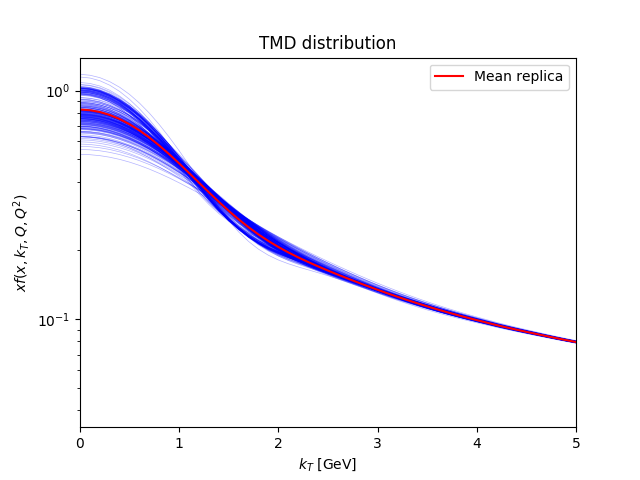
\includegraphics{pngplots/tmd_1_2_0.1.png}
\caption{TMD PDF of the \(d\) at \(Q = 2\) GeV and \(x = 0.1\)}
\end{figure}

\begin{figure}
\centering
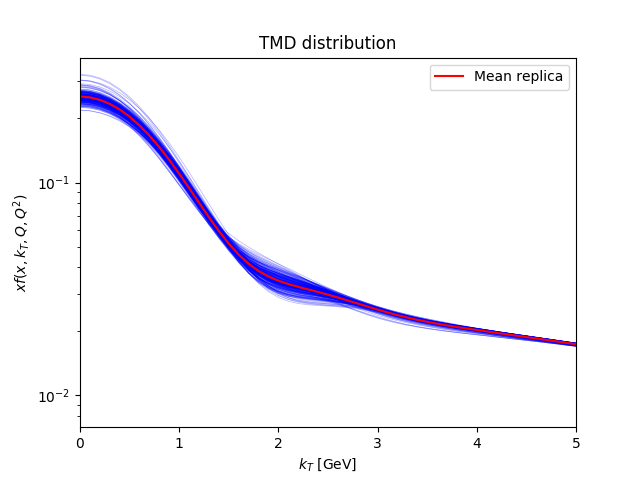
\includegraphics{pngplots/tmd_1_2_0.5.png}
\caption{TMD PDF of the \(d\) at \(Q = 2\) GeV and \(x = 0.5\)}
\end{figure}

\begin{figure}
\centering
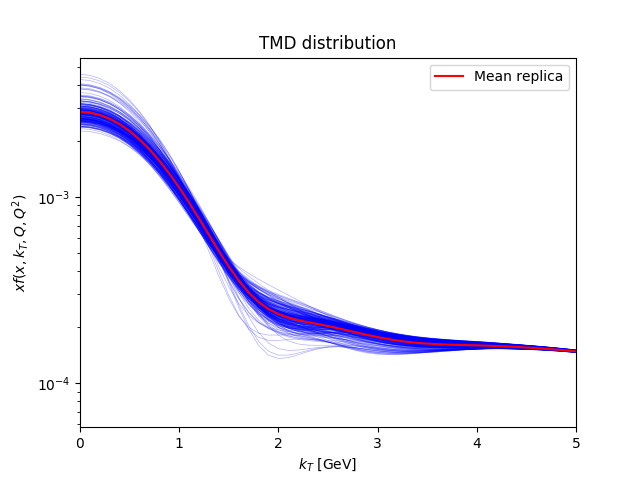
\includegraphics{pngplots/tmd_1_2_0.9.png}
\caption{TMD PDF of the \(d\) at \(Q = 2\) GeV and \(x = 0.9\)}
\end{figure}

\hypertarget{data-theory-comparison}{%
\subsection{Data-theory comparison}\label{data-theory-comparison}}

\begin{figure}
\centering
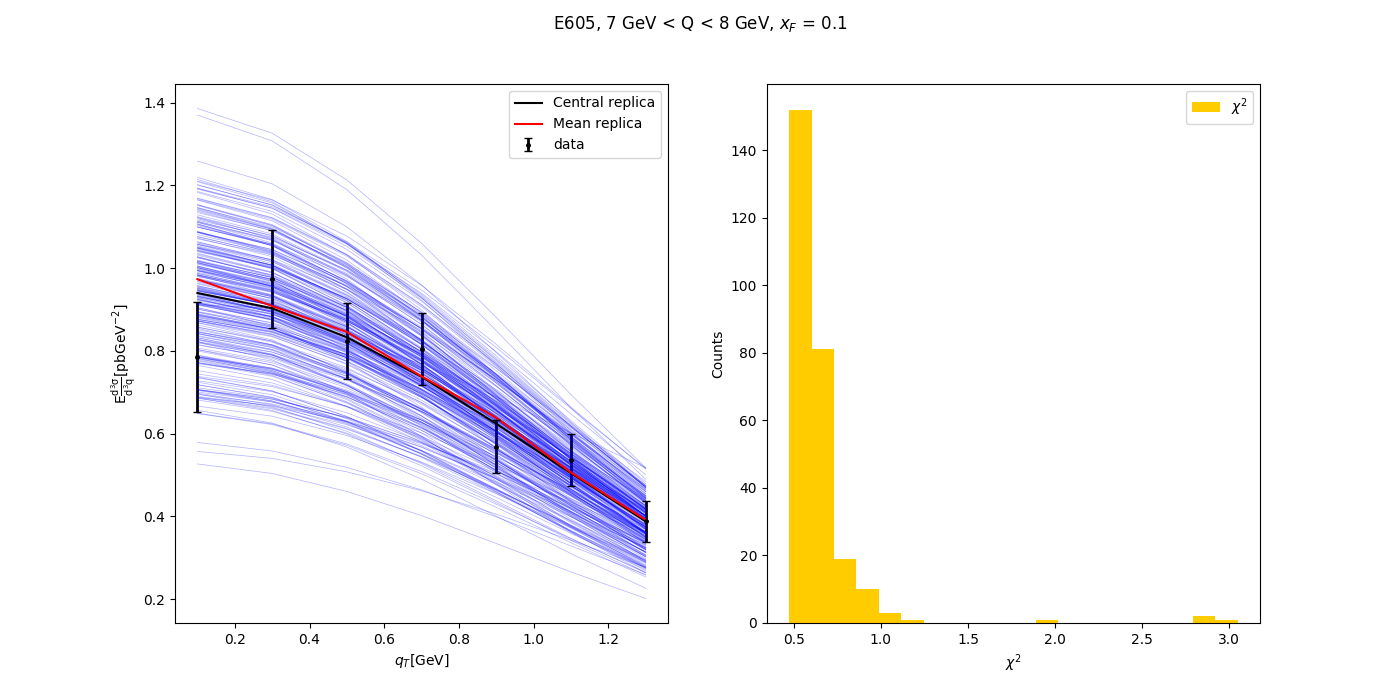
\includegraphics{pngplots/E605_Q_7_8.png}
\caption{E605\_Q\_7\_8 data-theory comparison}
\end{figure}

\begin{figure}
\centering
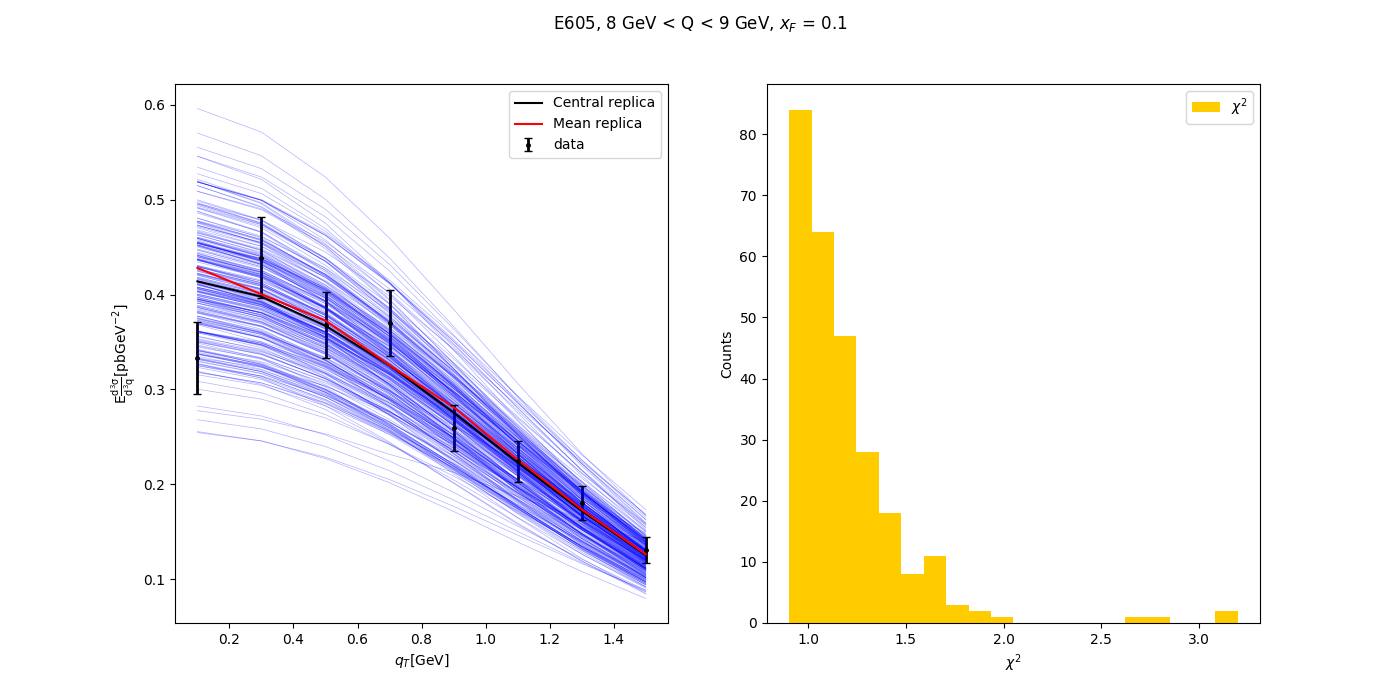
\includegraphics{pngplots/E605_Q_8_9.png}
\caption{E605\_Q\_8\_9 data-theory comparison}
\end{figure}

\begin{figure}
\centering
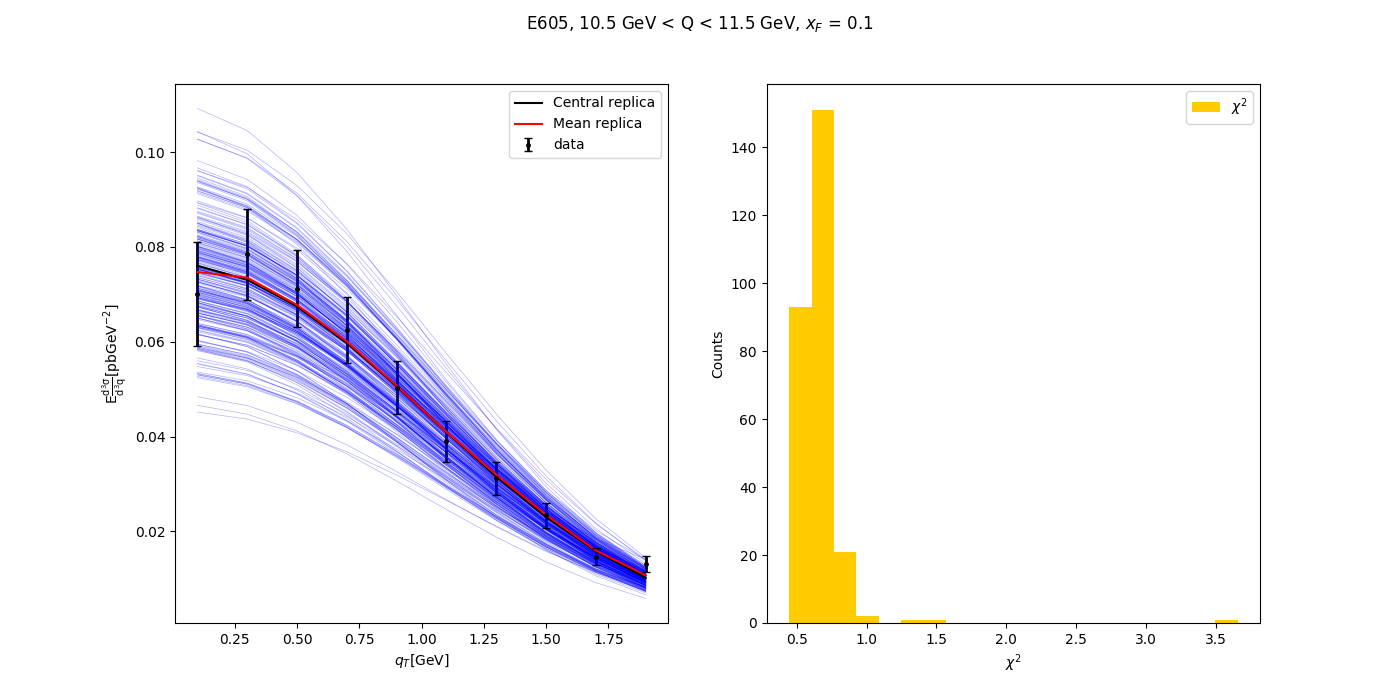
\includegraphics{pngplots/E605_Q_10.5_11.5.png}
\caption{E605\_Q\_10.5\_11.5 data-theory comparison}
\end{figure}

\begin{figure}
\centering
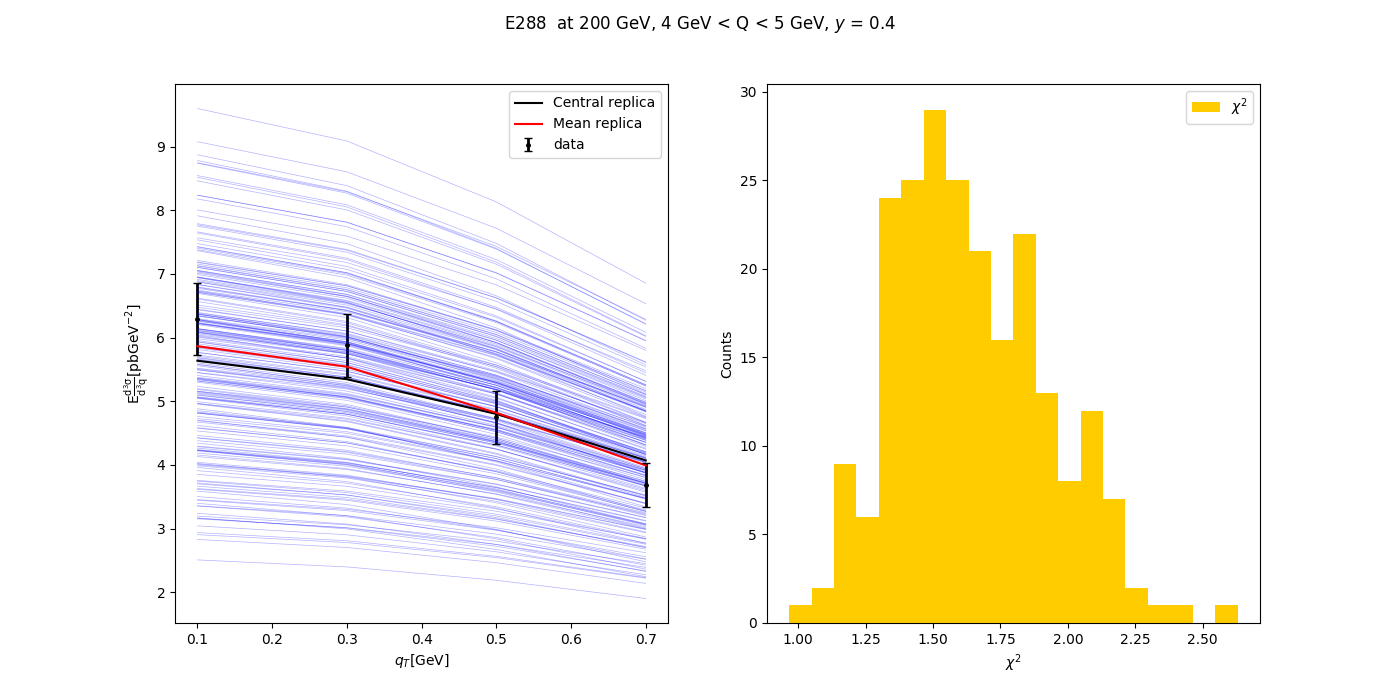
\includegraphics{pngplots/E288_200_Q_4_5.png}
\caption{E288\_200\_Q\_4\_5 data-theory comparison}
\end{figure}

\begin{figure}
\centering
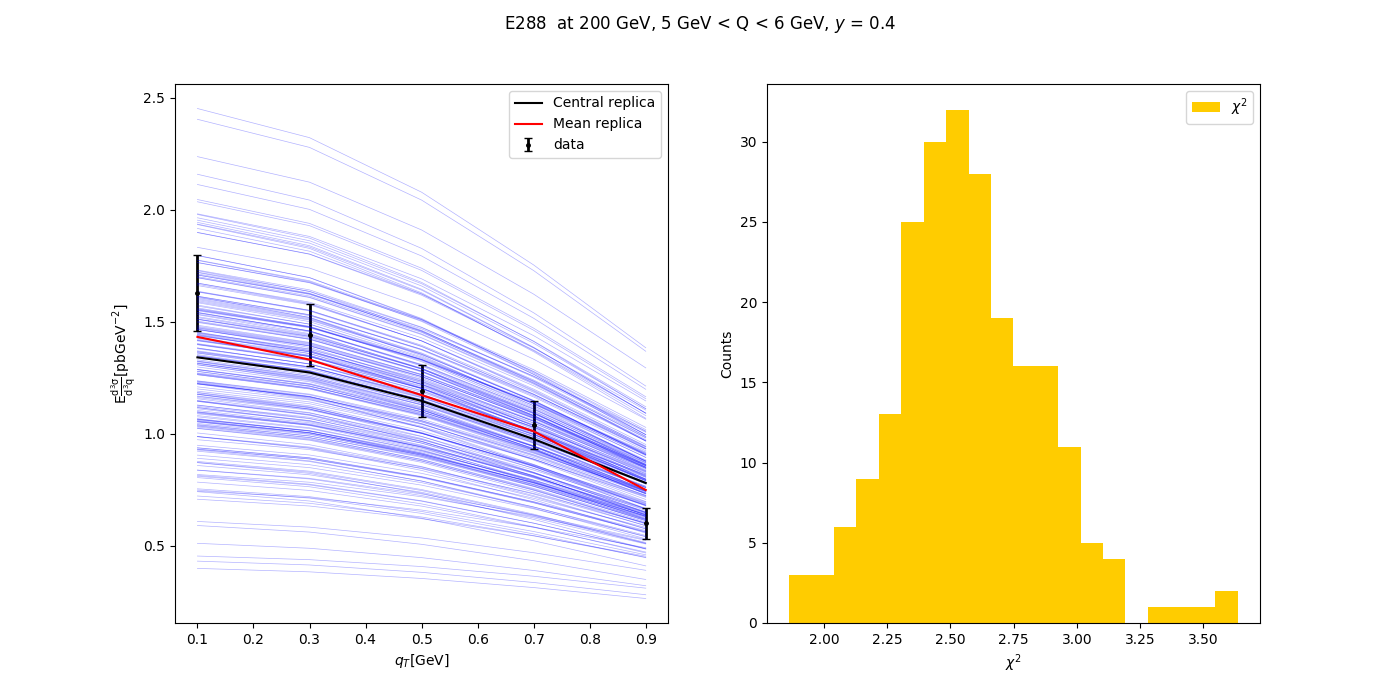
\includegraphics{pngplots/E288_200_Q_5_6.png}
\caption{E288\_200\_Q\_5\_6 data-theory comparison}
\end{figure}

\begin{figure}
\centering
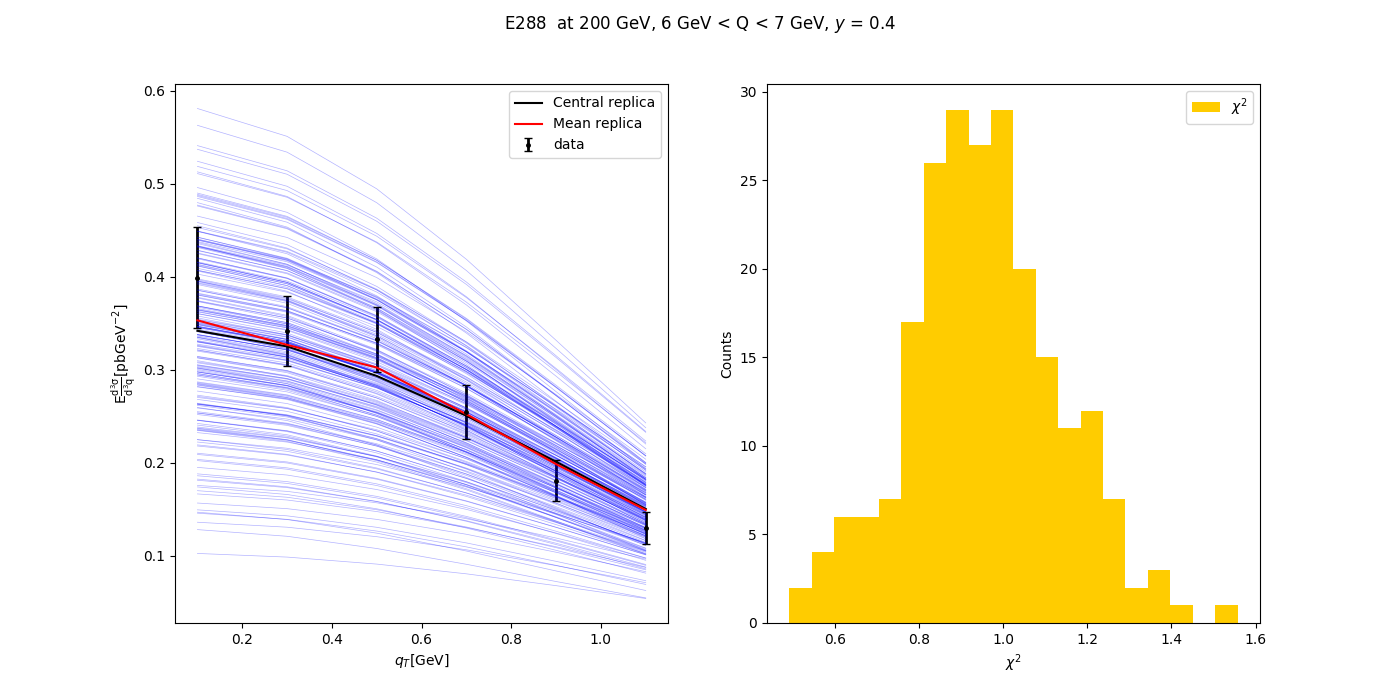
\includegraphics{pngplots/E288_200_Q_6_7.png}
\caption{E288\_200\_Q\_6\_7 data-theory comparison}
\end{figure}

\begin{figure}
\centering
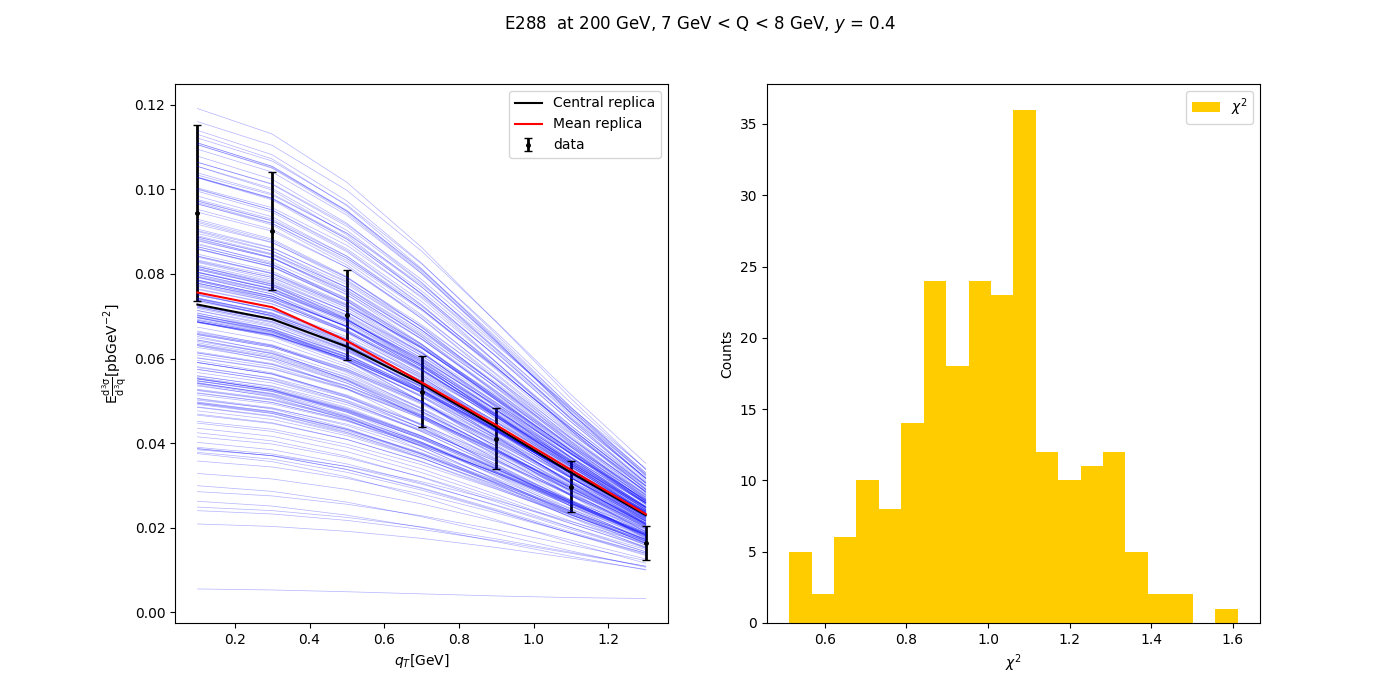
\includegraphics{pngplots/E288_200_Q_7_8.png}
\caption{E288\_200\_Q\_7\_8 data-theory comparison}
\end{figure}

\begin{figure}
\centering
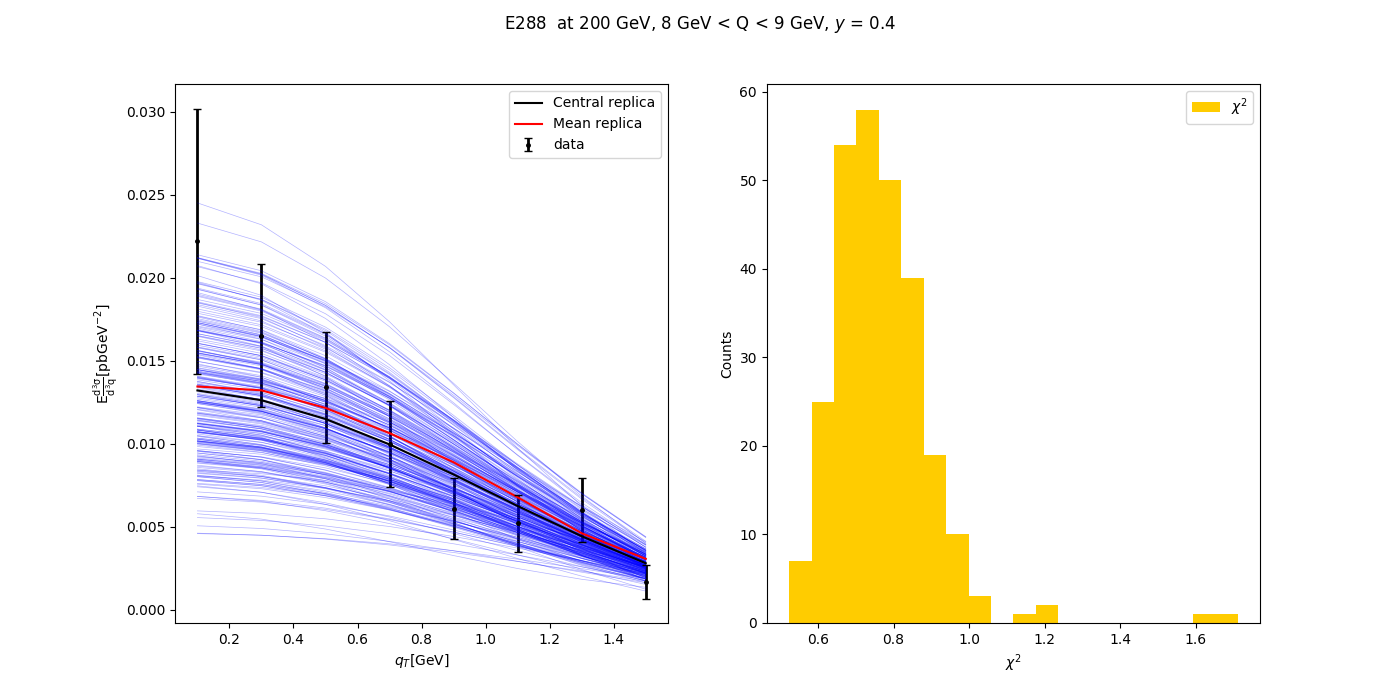
\includegraphics{pngplots/E288_200_Q_8_9.png}
\caption{E288\_200\_Q\_8\_9 data-theory comparison}
\end{figure}

\begin{figure}
\centering
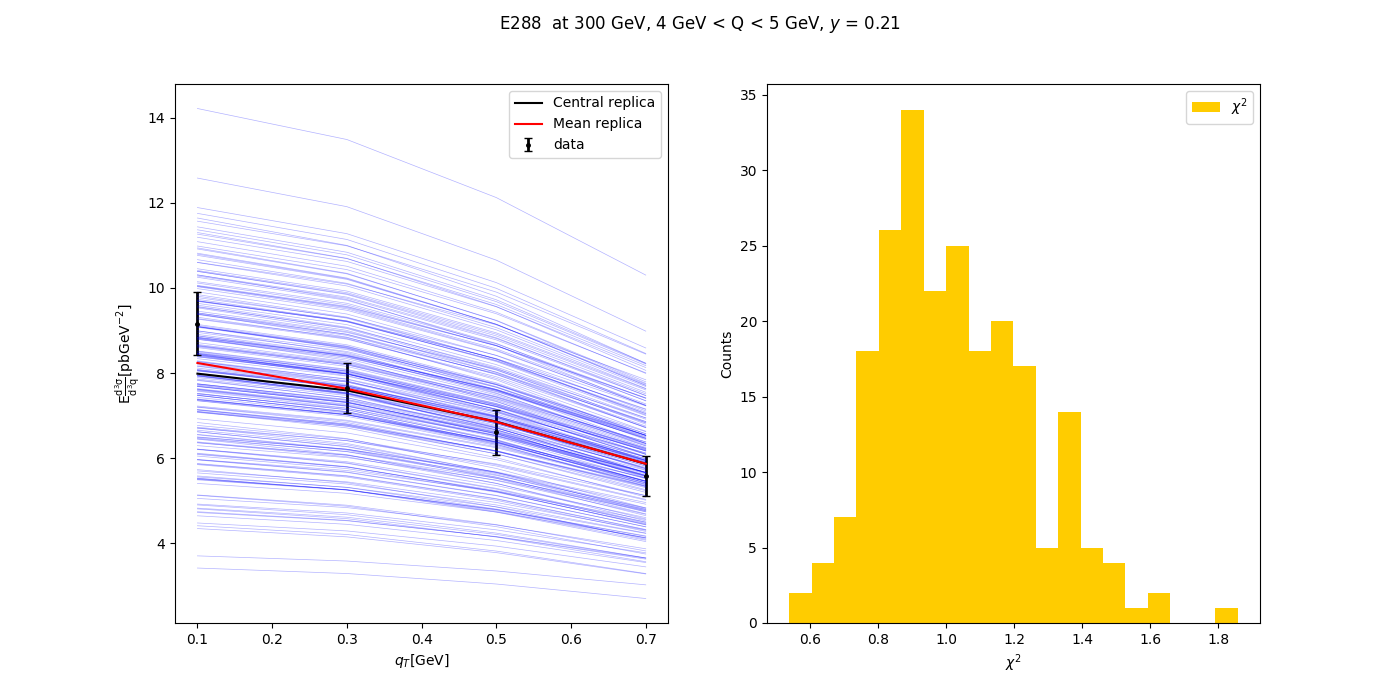
\includegraphics{pngplots/E288_300_Q_4_5.png}
\caption{E288\_300\_Q\_4\_5 data-theory comparison}
\end{figure}

\begin{figure}
\centering
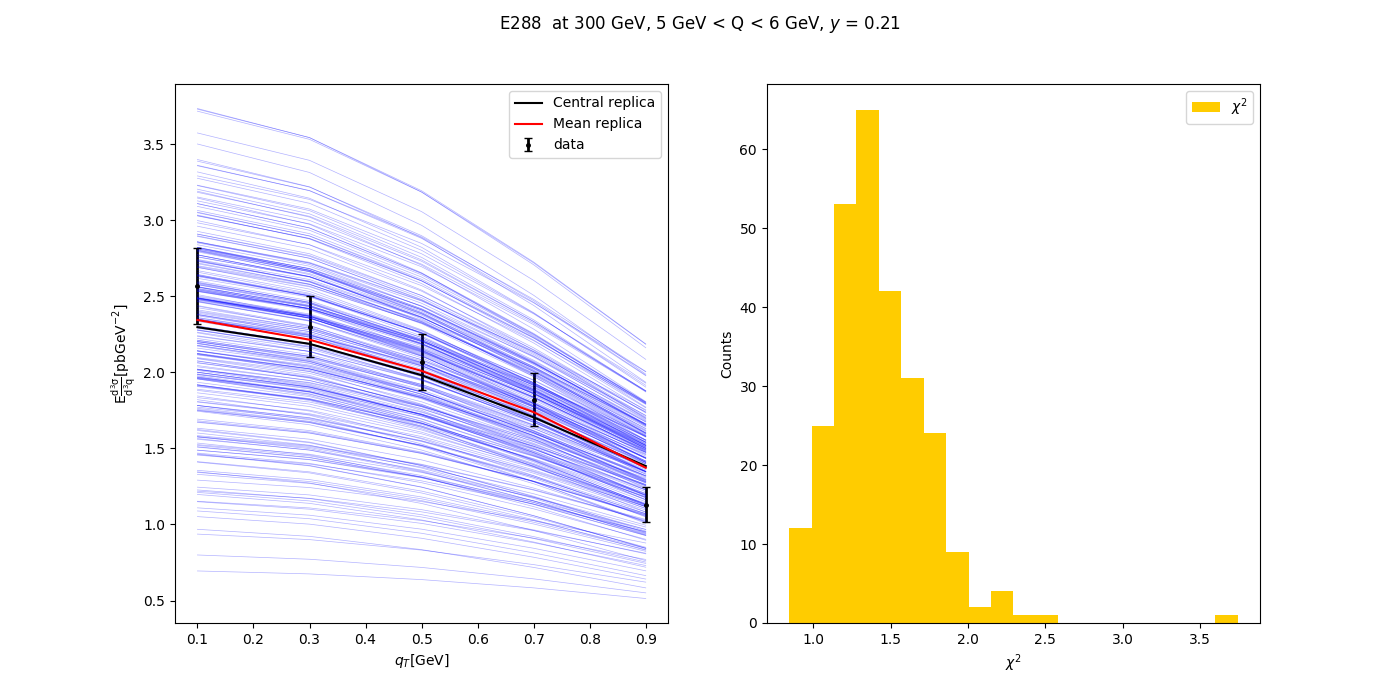
\includegraphics{pngplots/E288_300_Q_5_6.png}
\caption{E288\_300\_Q\_5\_6 data-theory comparison}
\end{figure}

\begin{figure}
\centering
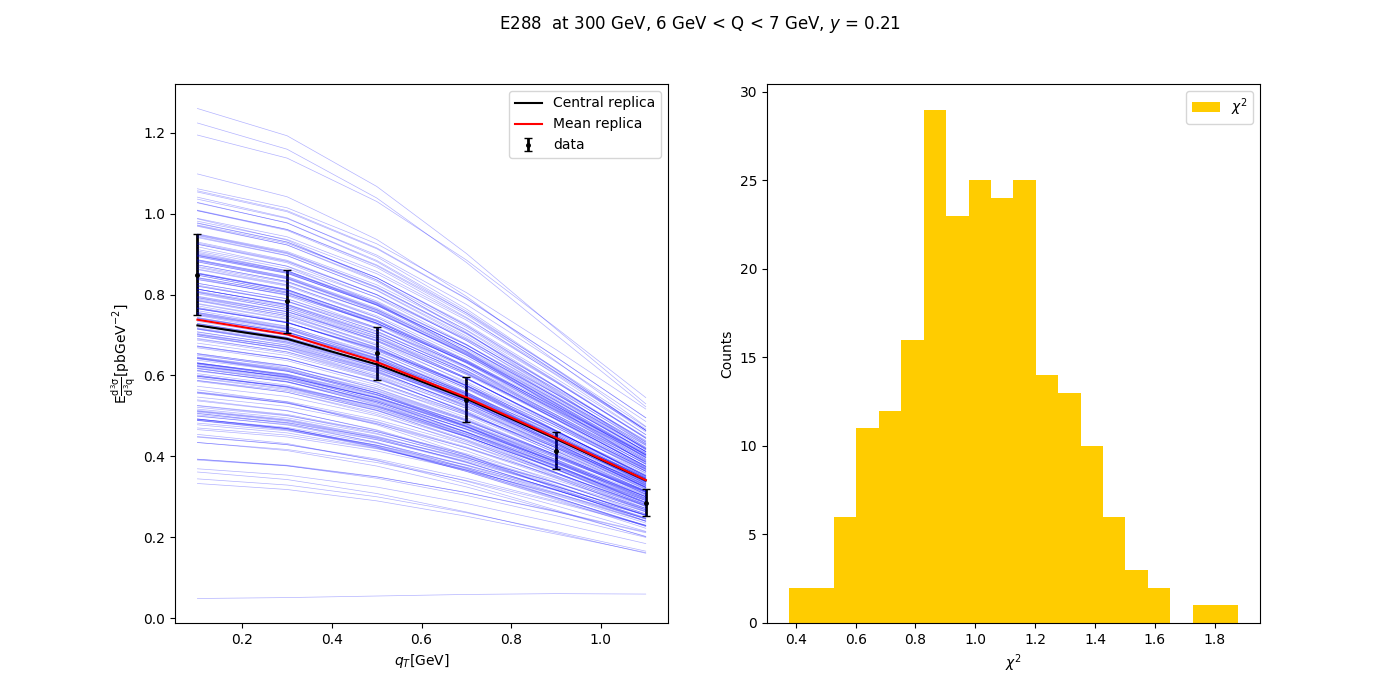
\includegraphics{pngplots/E288_300_Q_6_7.png}
\caption{E288\_300\_Q\_6\_7 data-theory comparison}
\end{figure}

\begin{figure}
\centering
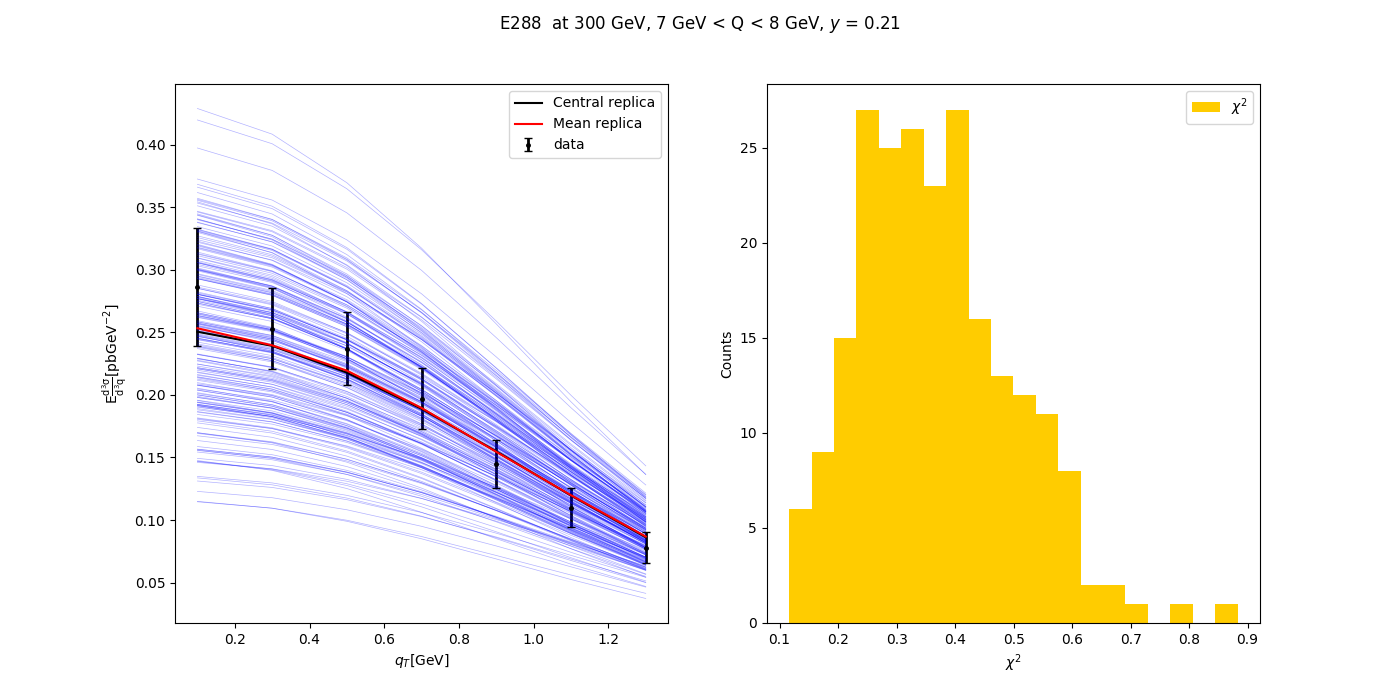
\includegraphics{pngplots/E288_300_Q_7_8.png}
\caption{E288\_300\_Q\_7\_8 data-theory comparison}
\end{figure}

\begin{figure}
\centering
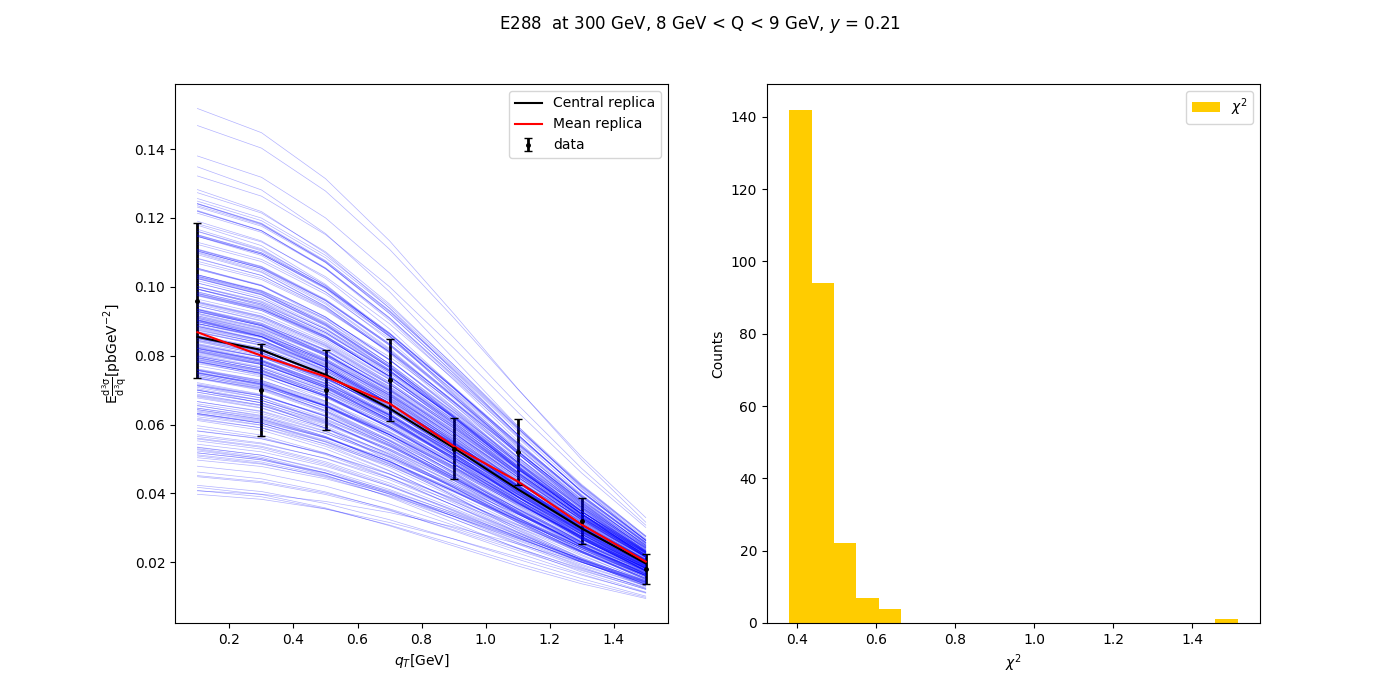
\includegraphics{pngplots/E288_300_Q_8_9.png}
\caption{E288\_300\_Q\_8\_9 data-theory comparison}
\end{figure}

\begin{figure}
\centering
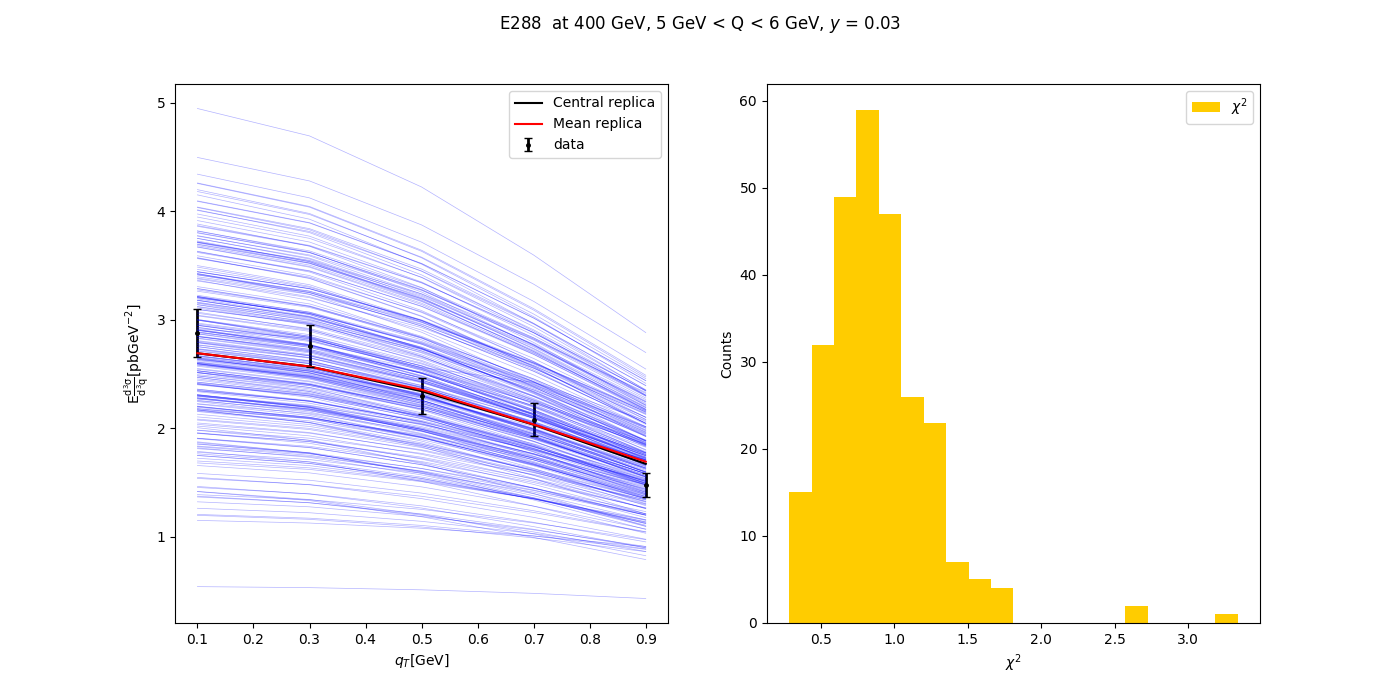
\includegraphics{pngplots/E288_400_Q_5_6.png}
\caption{E288\_400\_Q\_5\_6 data-theory comparison}
\end{figure}

\begin{figure}
\centering
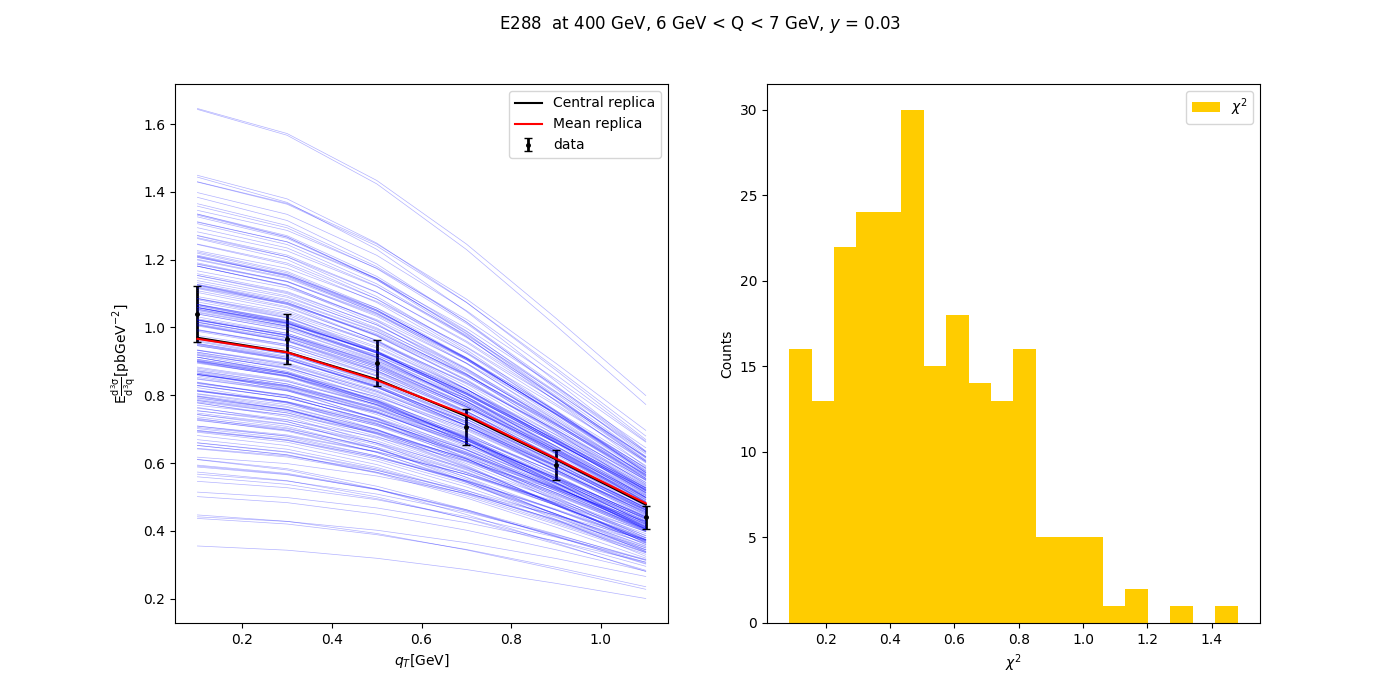
\includegraphics{pngplots/E288_400_Q_6_7.png}
\caption{E288\_400\_Q\_6\_7 data-theory comparison}
\end{figure}

\begin{figure}
\centering
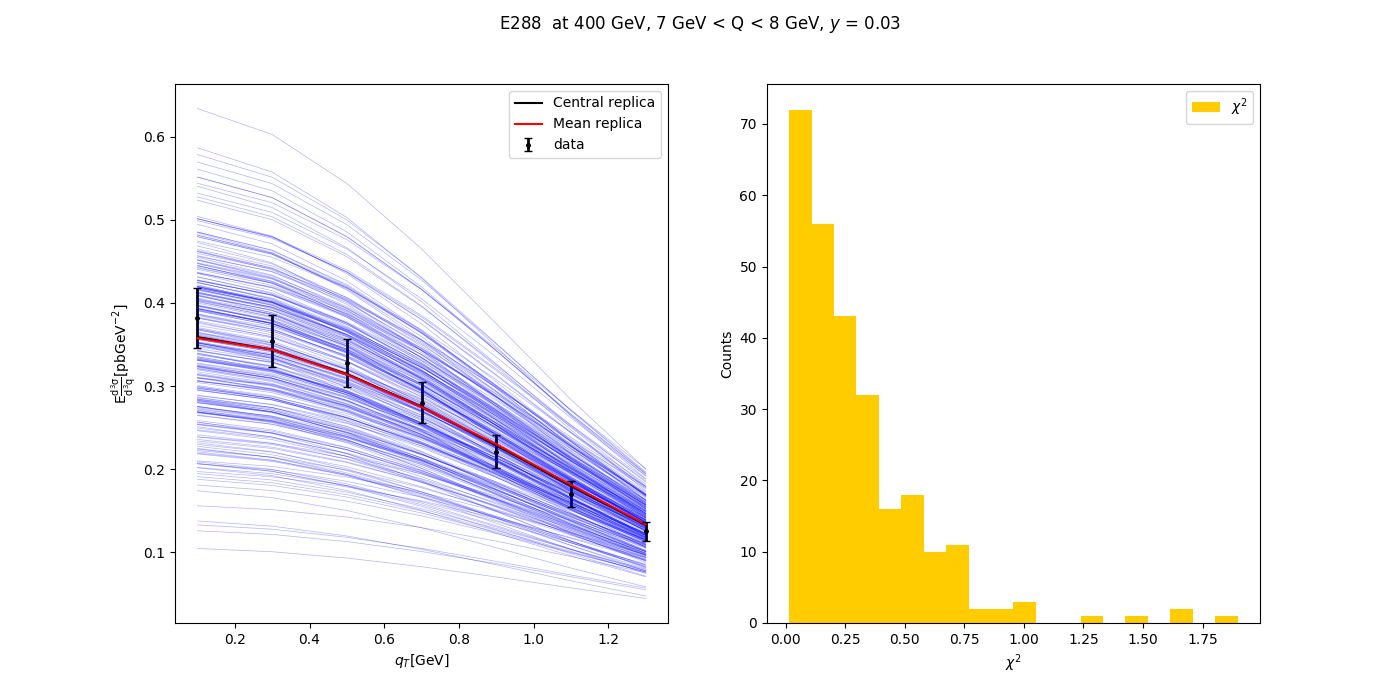
\includegraphics{pngplots/E288_400_Q_7_8.png}
\caption{E288\_400\_Q\_7\_8 data-theory comparison}
\end{figure}

\begin{figure}
\centering
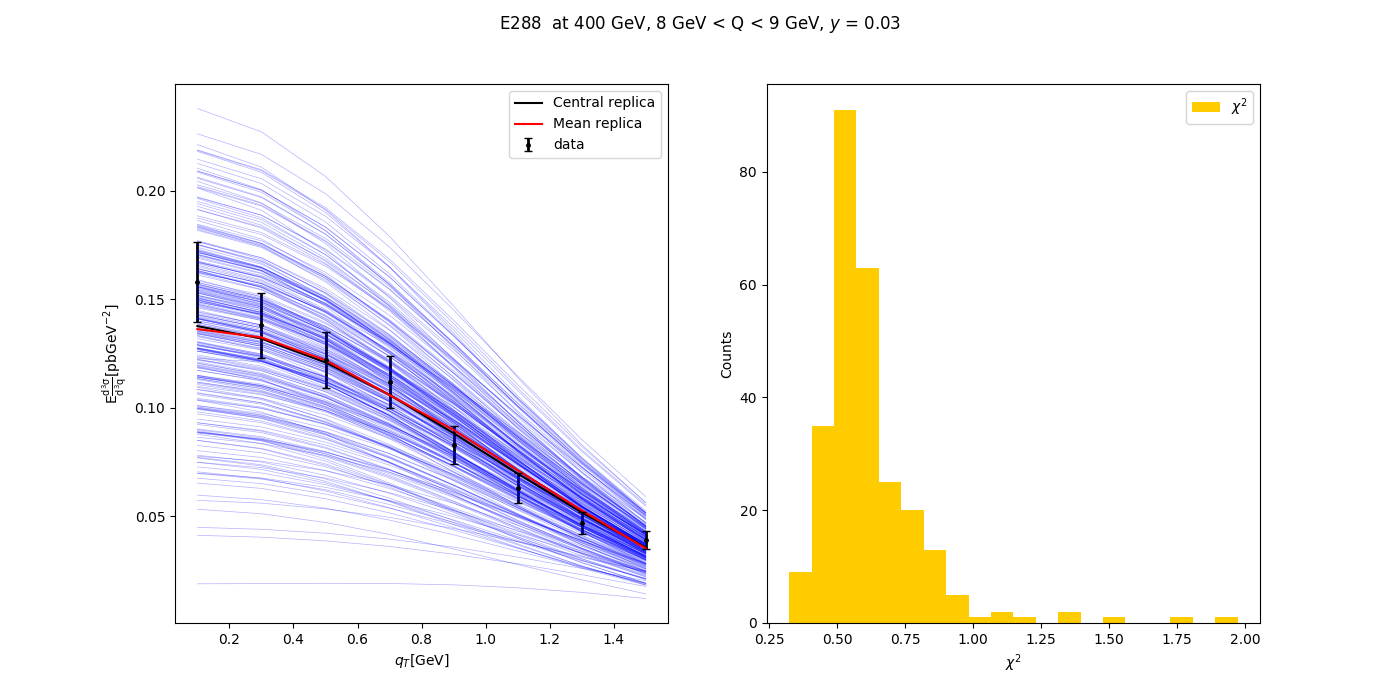
\includegraphics{pngplots/E288_400_Q_8_9.png}
\caption{E288\_400\_Q\_8\_9 data-theory comparison}
\end{figure}

\begin{figure}
\centering
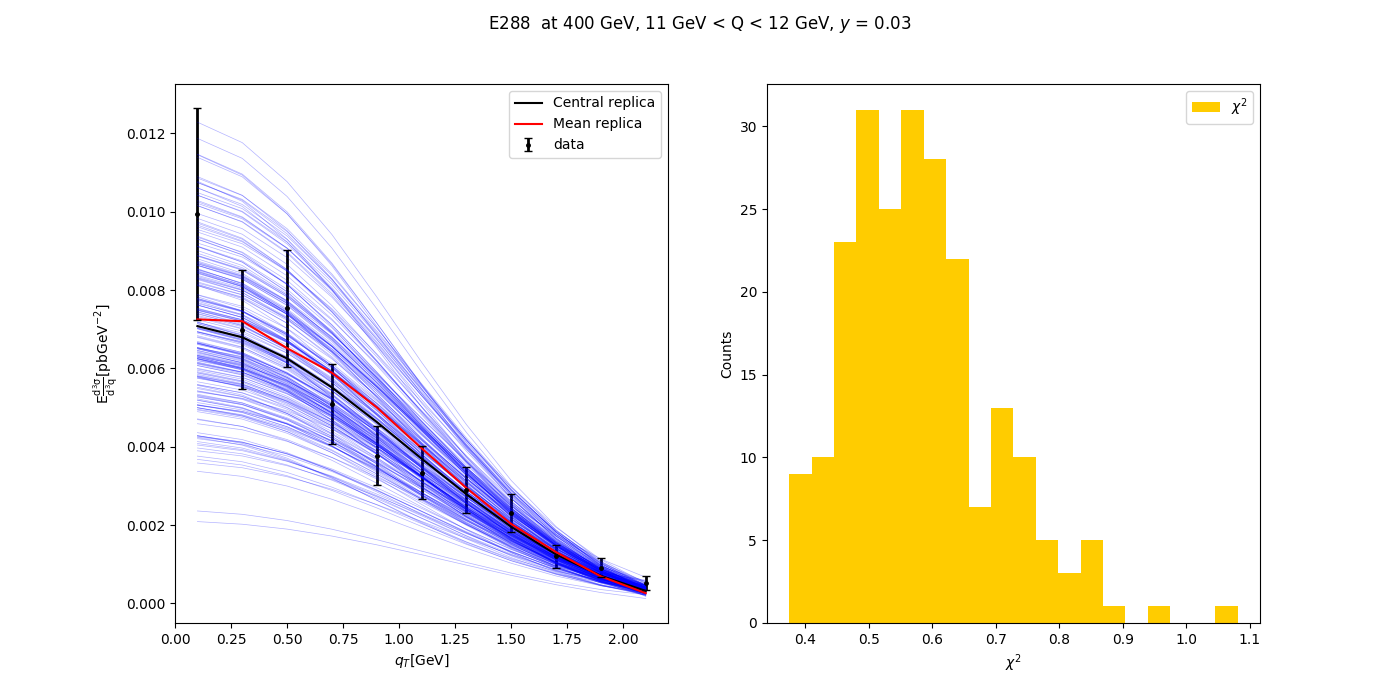
\includegraphics{pngplots/E288_400_Q_11_12.png}
\caption{E288\_400\_Q\_11\_12 data-theory comparison}
\end{figure}

\begin{figure}
\centering
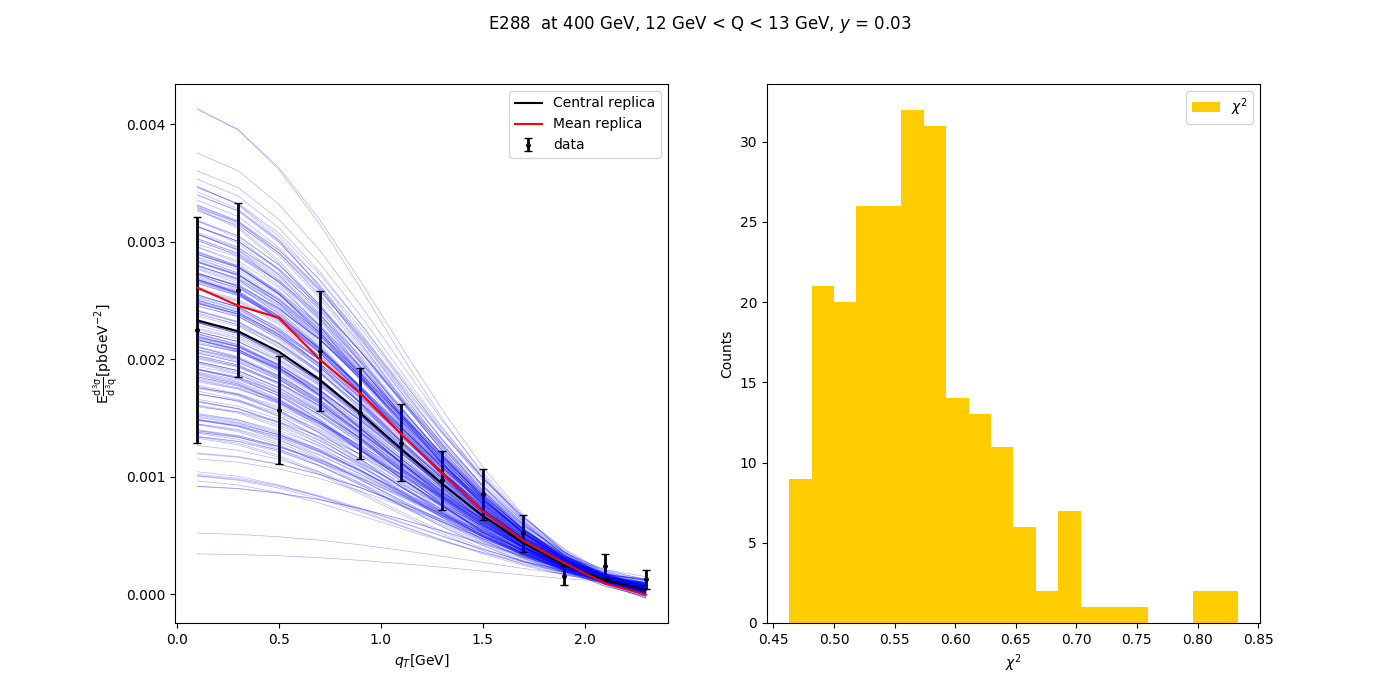
\includegraphics{pngplots/E288_400_Q_12_13.png}
\caption{E288\_400\_Q\_12\_13 data-theory comparison}
\end{figure}

\begin{figure}
\centering
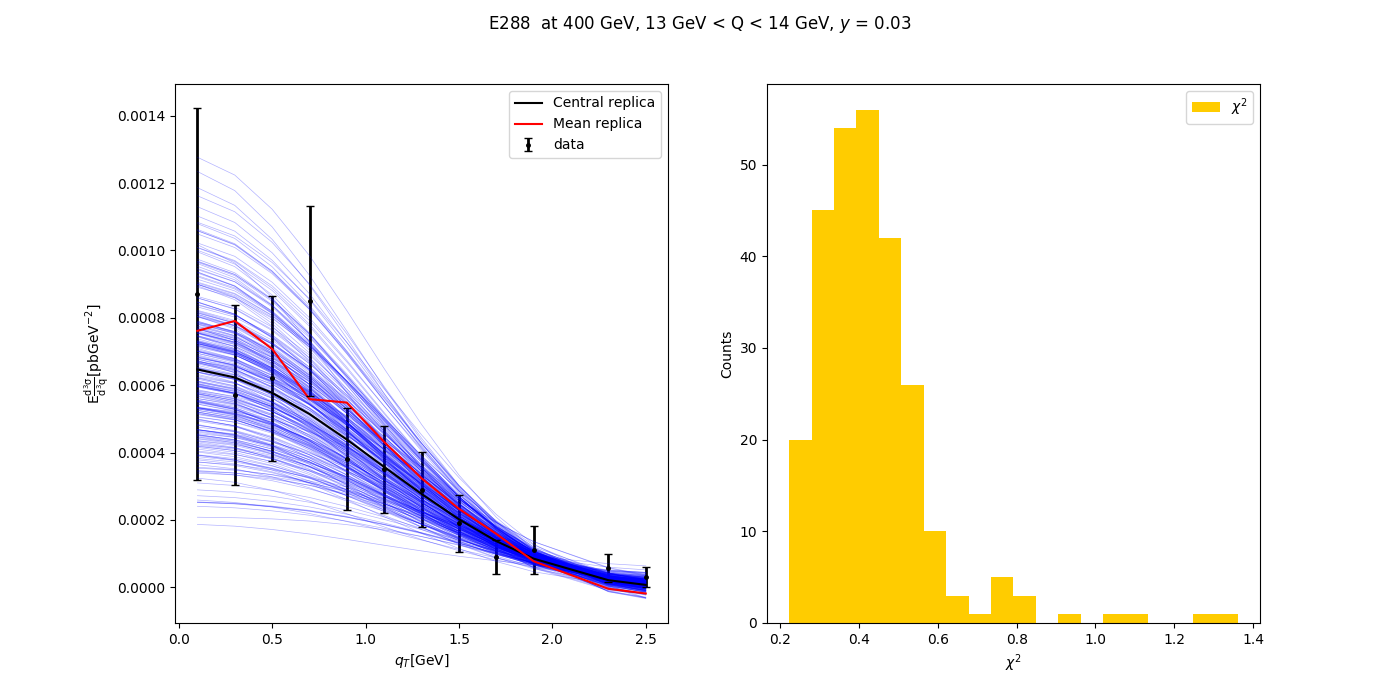
\includegraphics{pngplots/E288_400_Q_13_14.png}
\caption{E288\_400\_Q\_13\_14 data-theory comparison}
\end{figure}

\begin{figure}
\centering
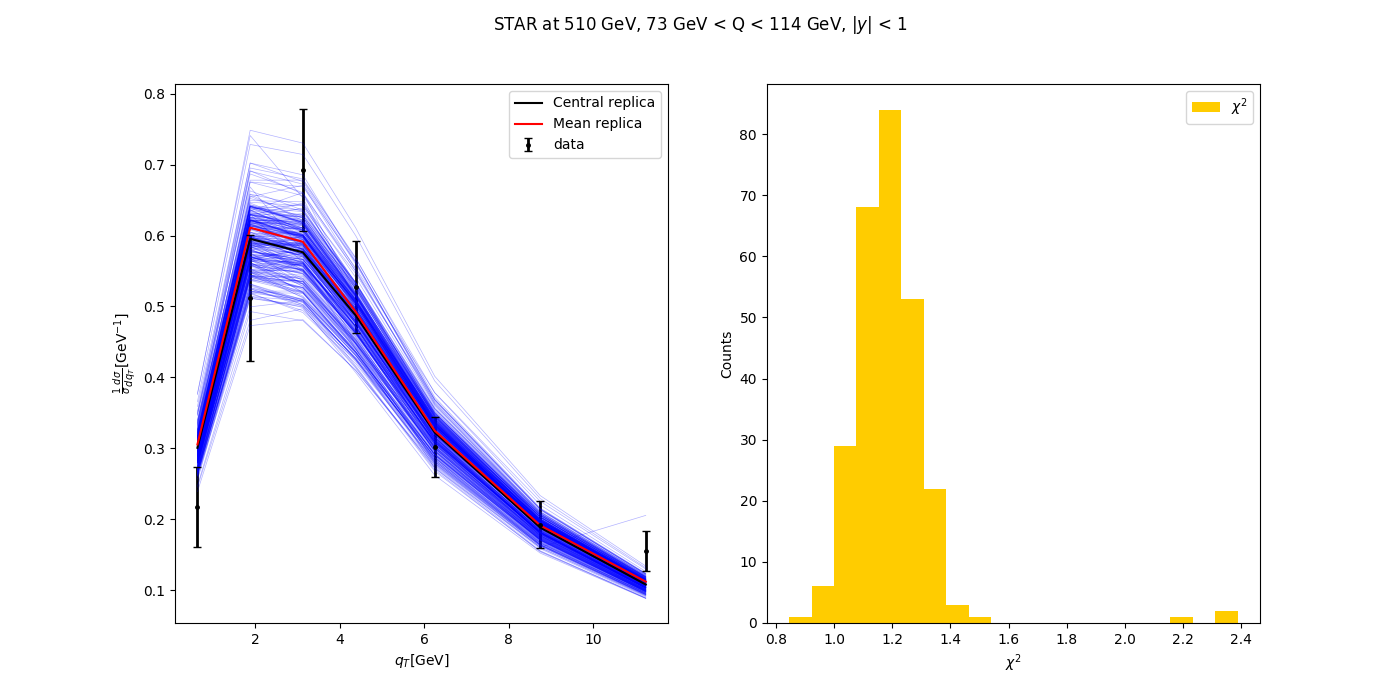
\includegraphics{pngplots/STAR_510.png}
\caption{STAR\_510 data-theory comparison}
\end{figure}

\begin{figure}
\centering
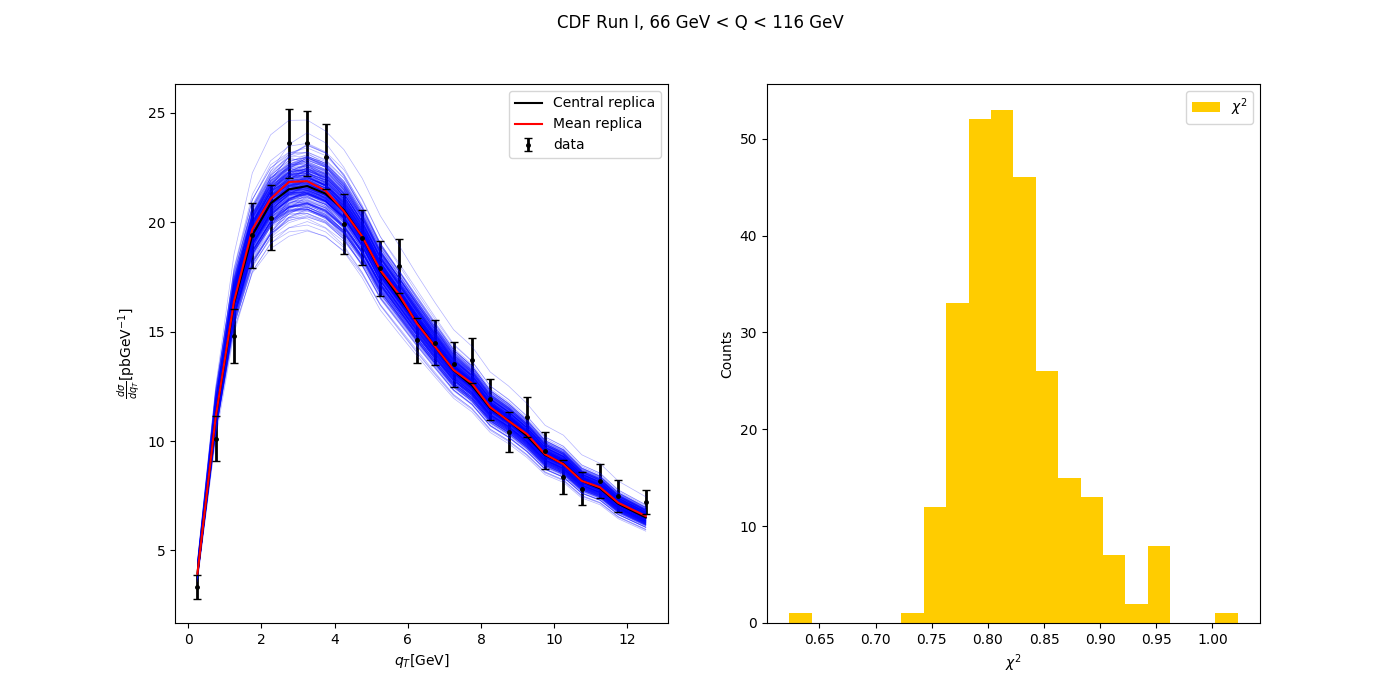
\includegraphics{pngplots/CDF_RunI.png}
\caption{CDF\_RunI data-theory comparison}
\end{figure}

\begin{figure}
\centering
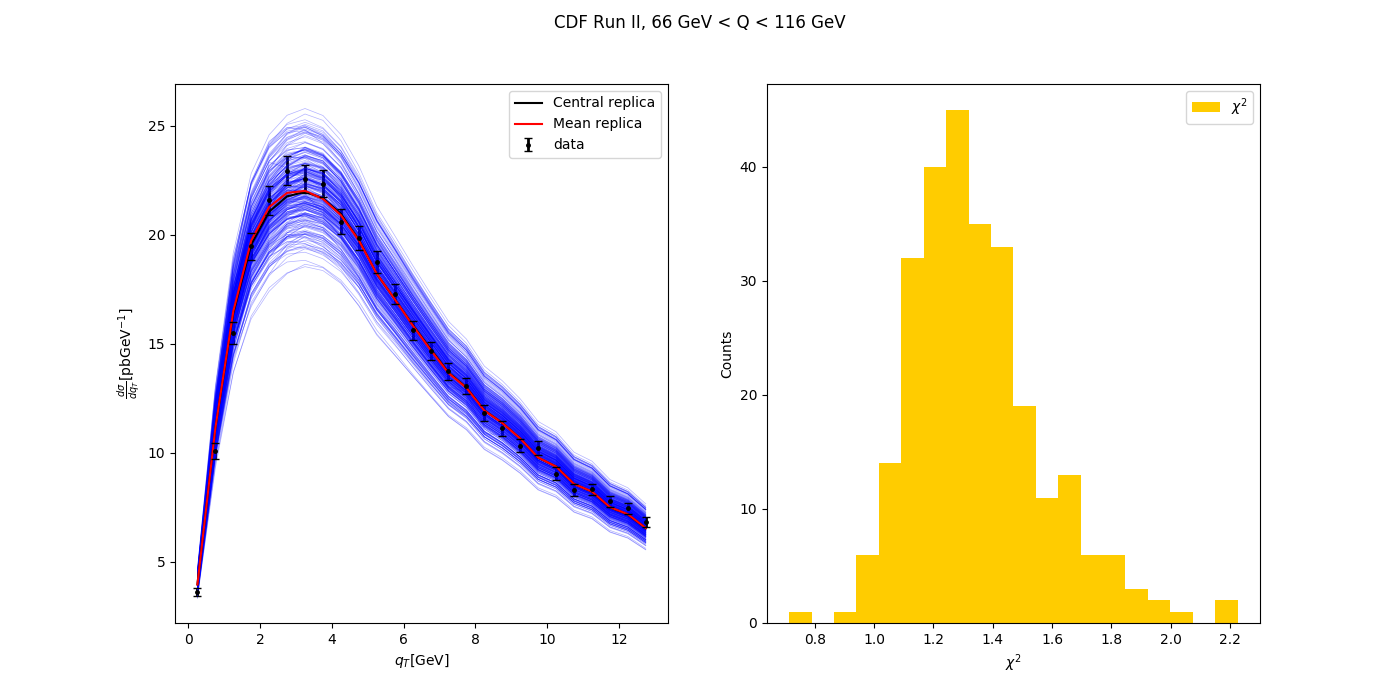
\includegraphics{pngplots/CDF_RunII.png}
\caption{CDF\_RunII data-theory comparison}
\end{figure}

\begin{figure}
\centering
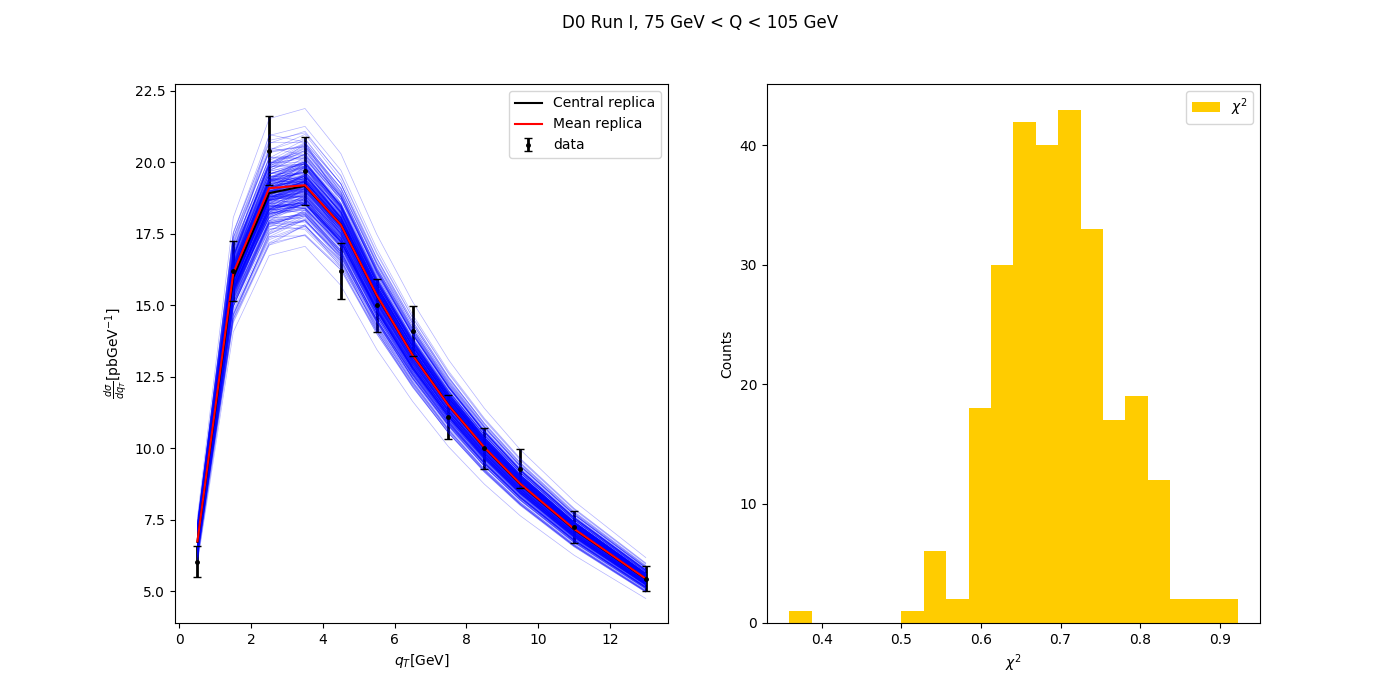
\includegraphics{pngplots/D0_RunI.png}
\caption{D0\_RunI data-theory comparison}
\end{figure}

\begin{figure}
\centering
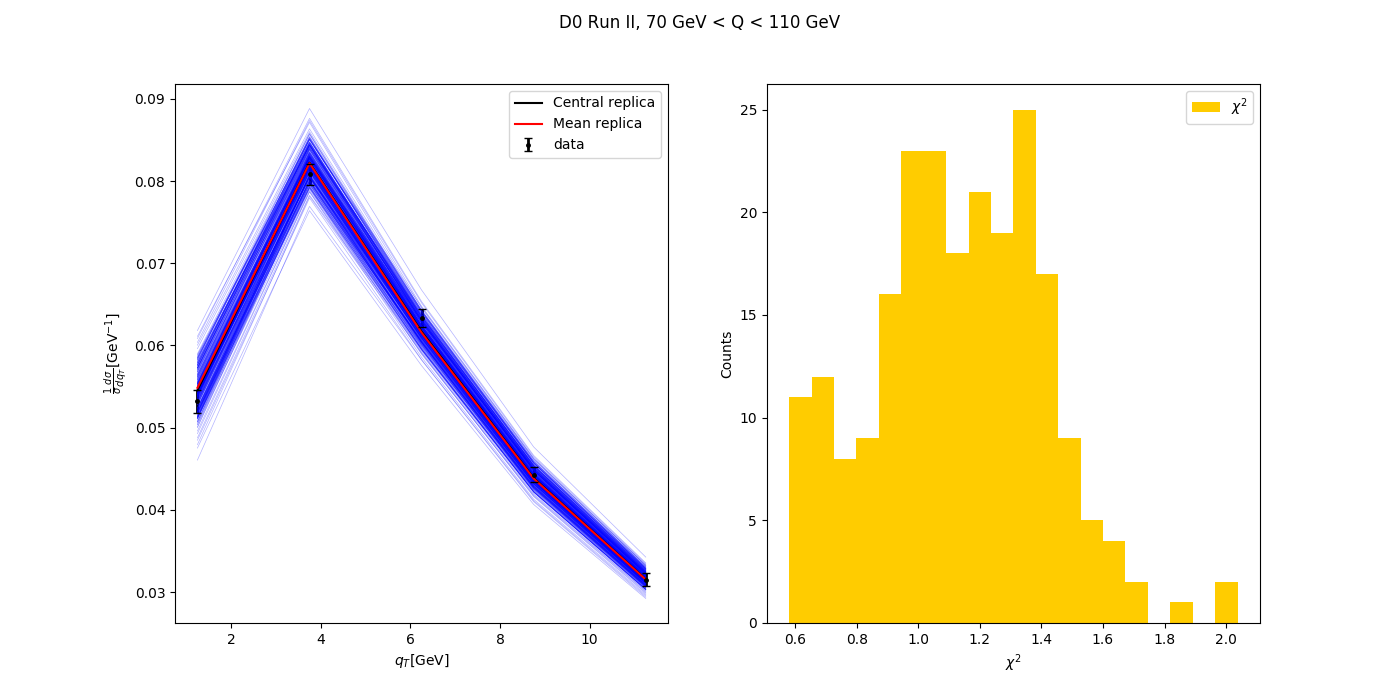
\includegraphics{pngplots/D0_RunII.png}
\caption{D0\_RunII data-theory comparison}
\end{figure}

\begin{figure}
\centering
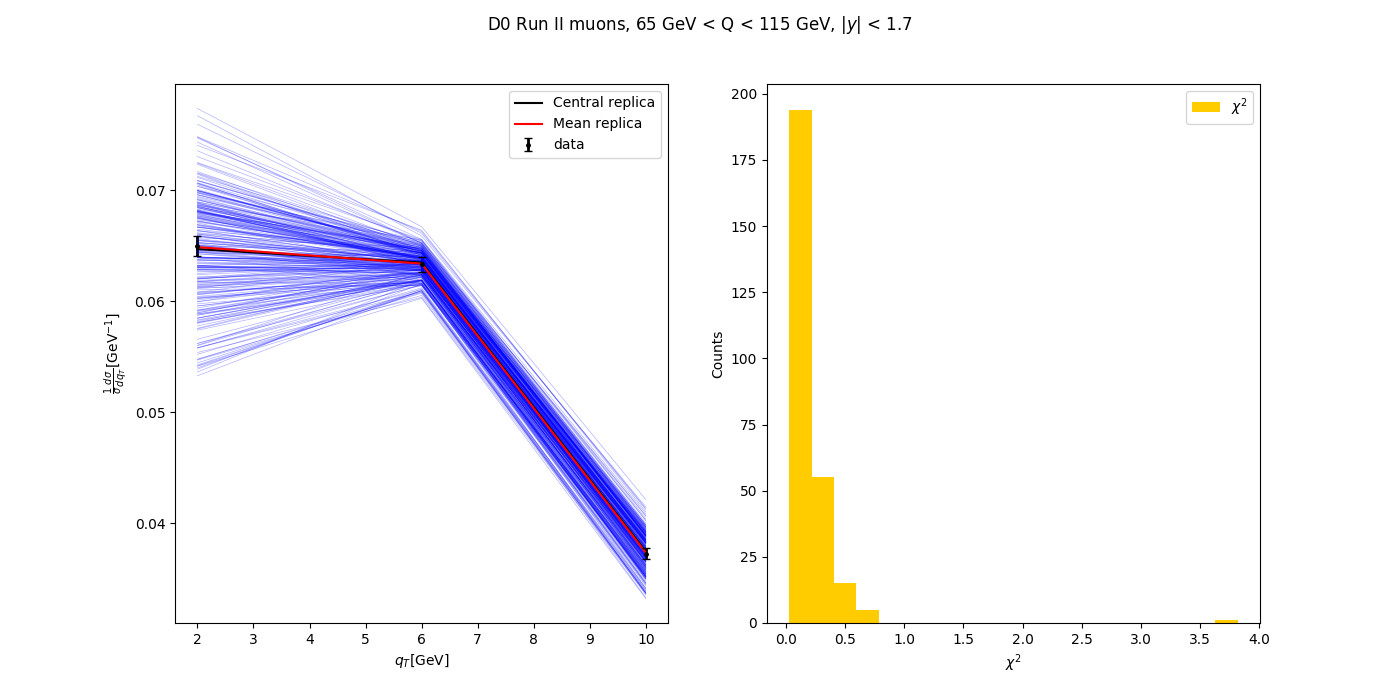
\includegraphics{pngplots/D0_RunIImu.png}
\caption{D0\_RunIImu data-theory comparison}
\end{figure}

\begin{figure}
\centering
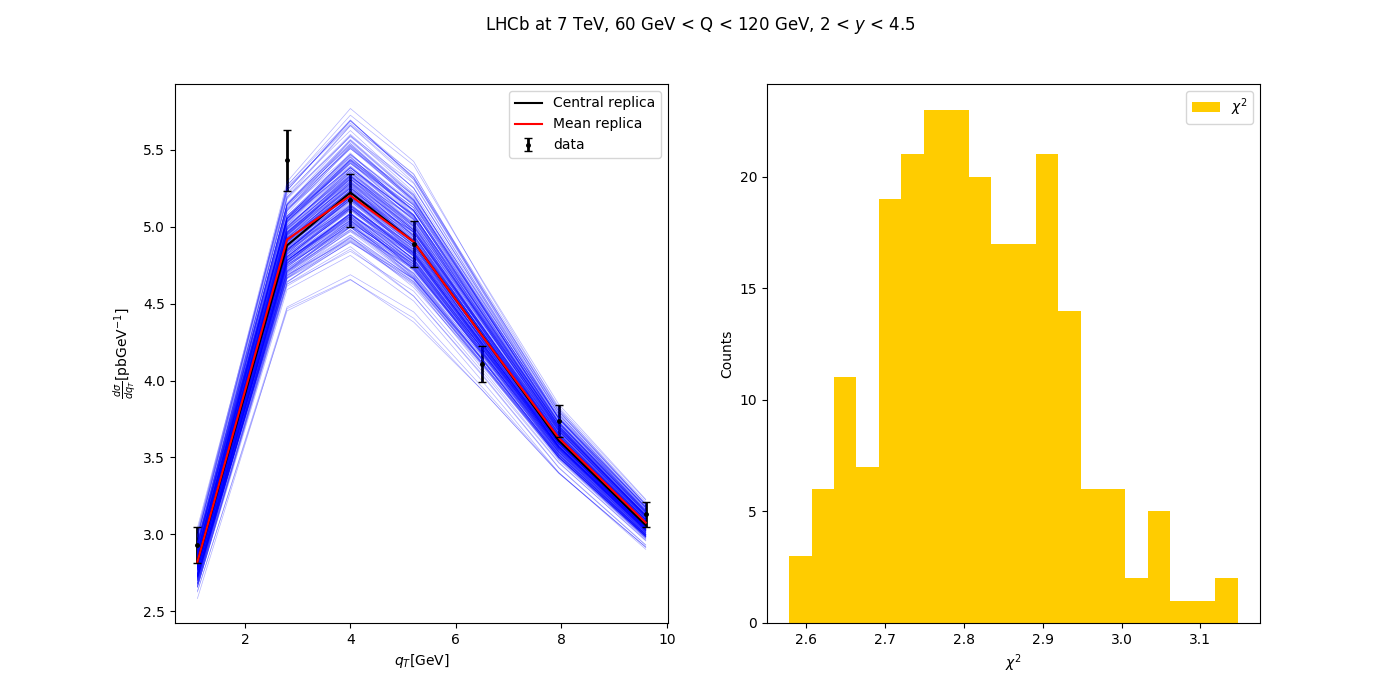
\includegraphics{pngplots/LHCb_7TeV.png}
\caption{LHCb\_7TeV data-theory comparison}
\end{figure}

\begin{figure}
\centering
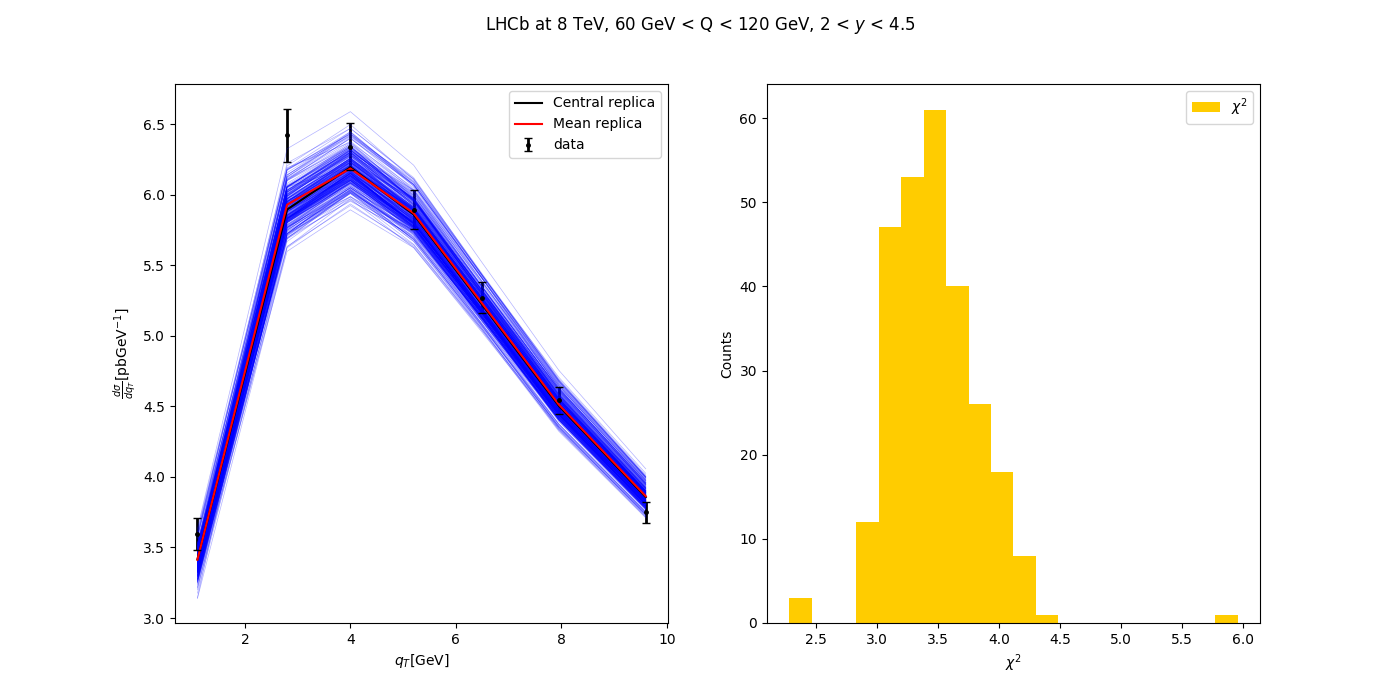
\includegraphics{pngplots/LHCb_8TeV.png}
\caption{LHCb\_8TeV data-theory comparison}
\end{figure}

\begin{figure}
\centering
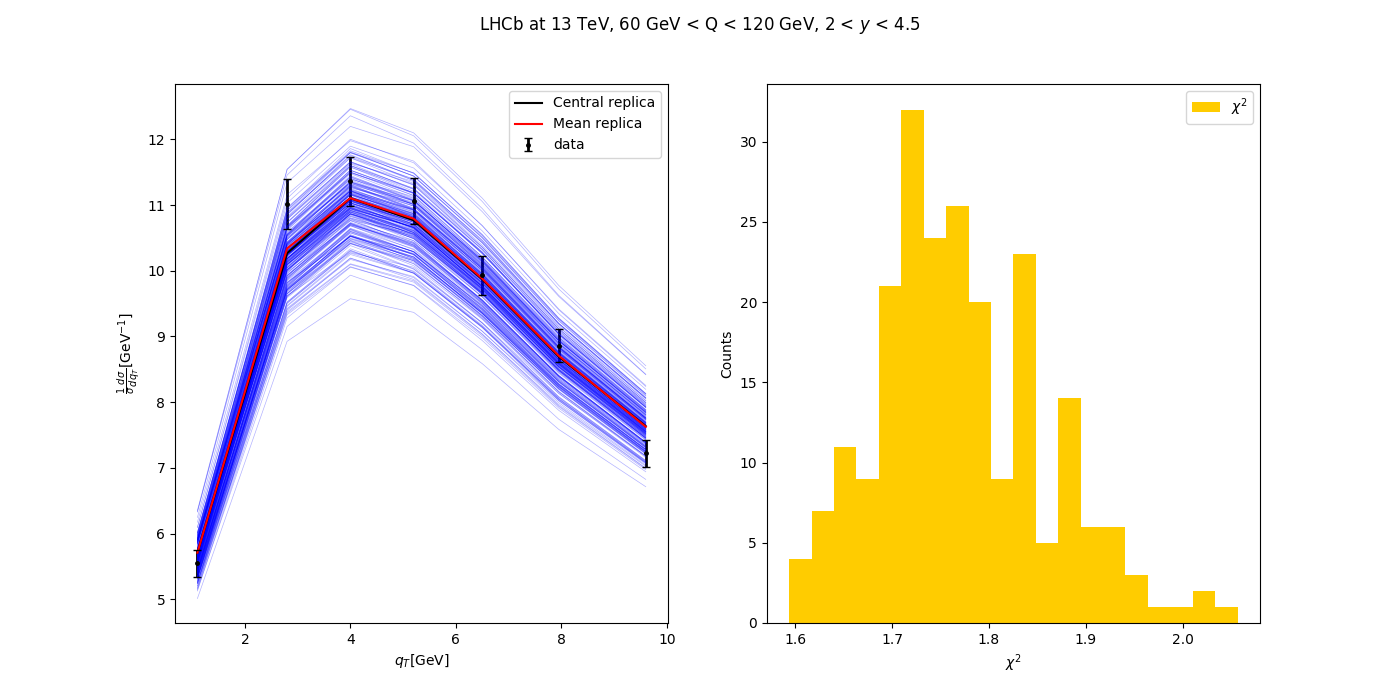
\includegraphics{pngplots/LHCb_13TeV.png}
\caption{LHCb\_13TeV data-theory comparison}
\end{figure}

\begin{figure}
\centering
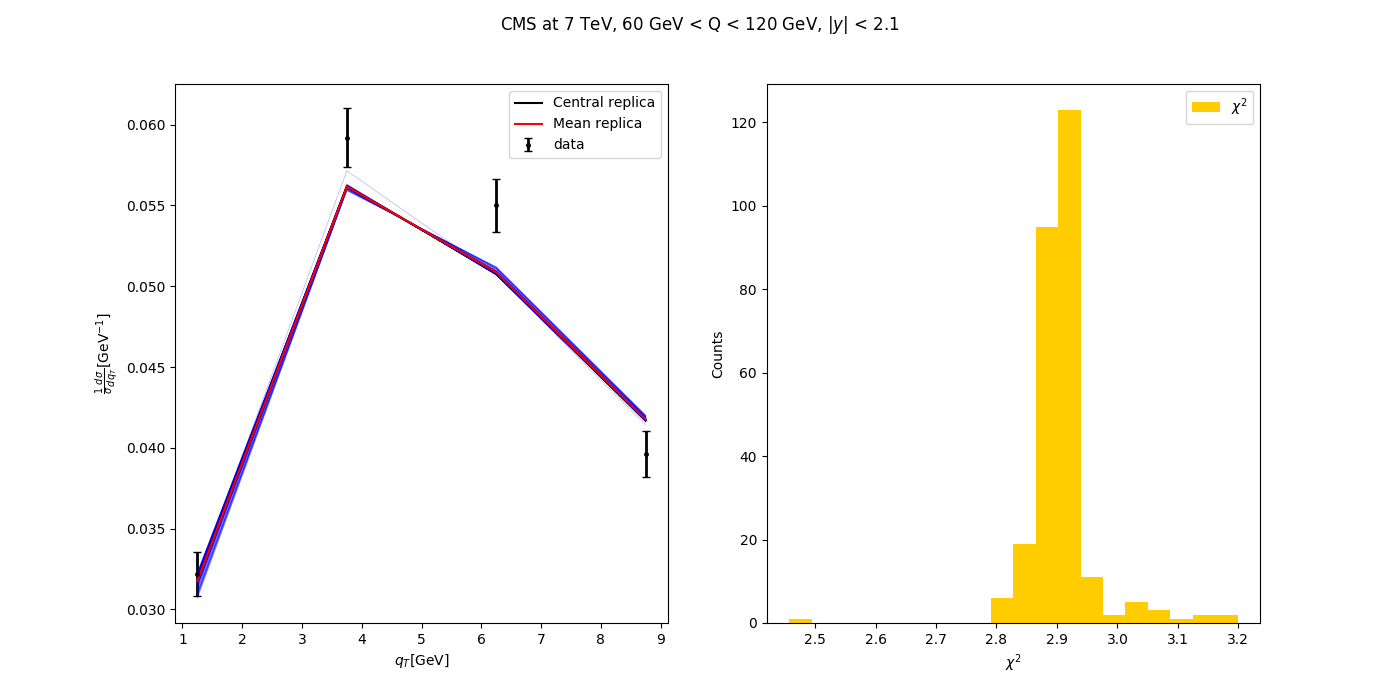
\includegraphics{pngplots/CMS_7TeV.png}
\caption{CMS\_7TeV data-theory comparison}
\end{figure}

\begin{figure}
\centering
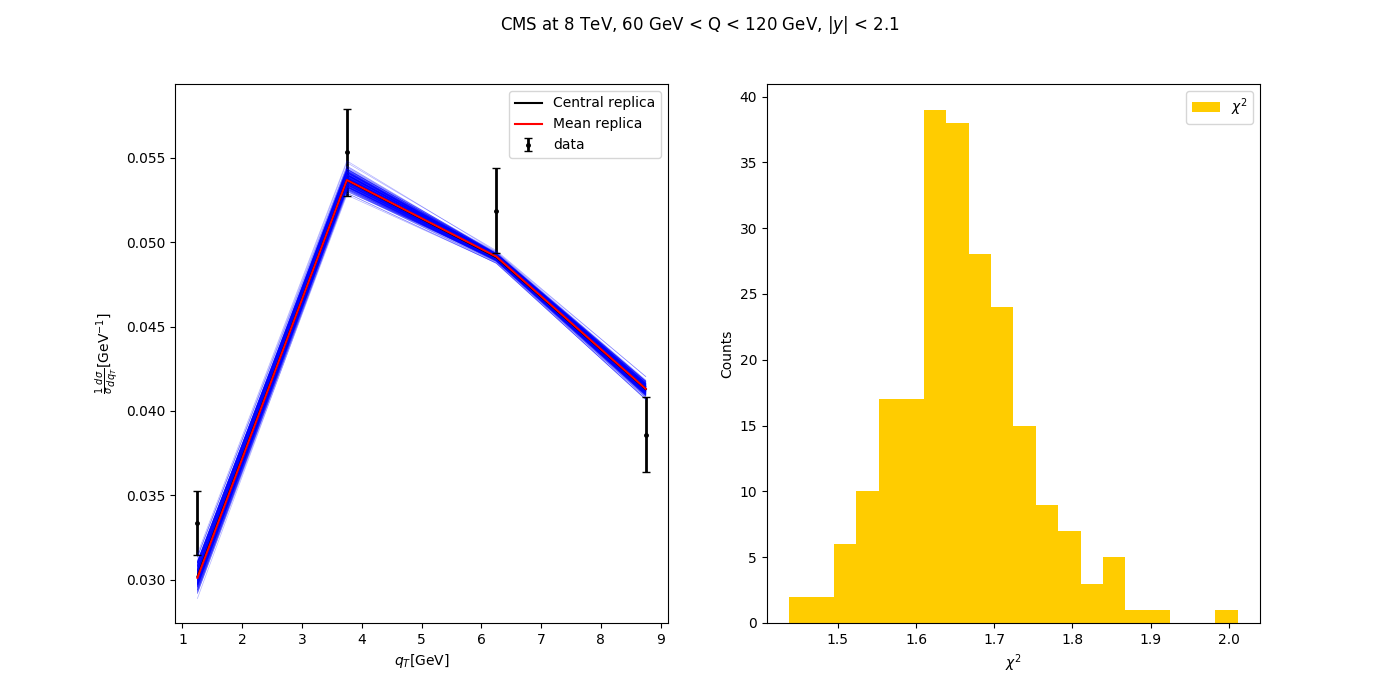
\includegraphics{pngplots/CMS_8TeV.png}
\caption{CMS\_8TeV data-theory comparison}
\end{figure}

\begin{figure}
\centering
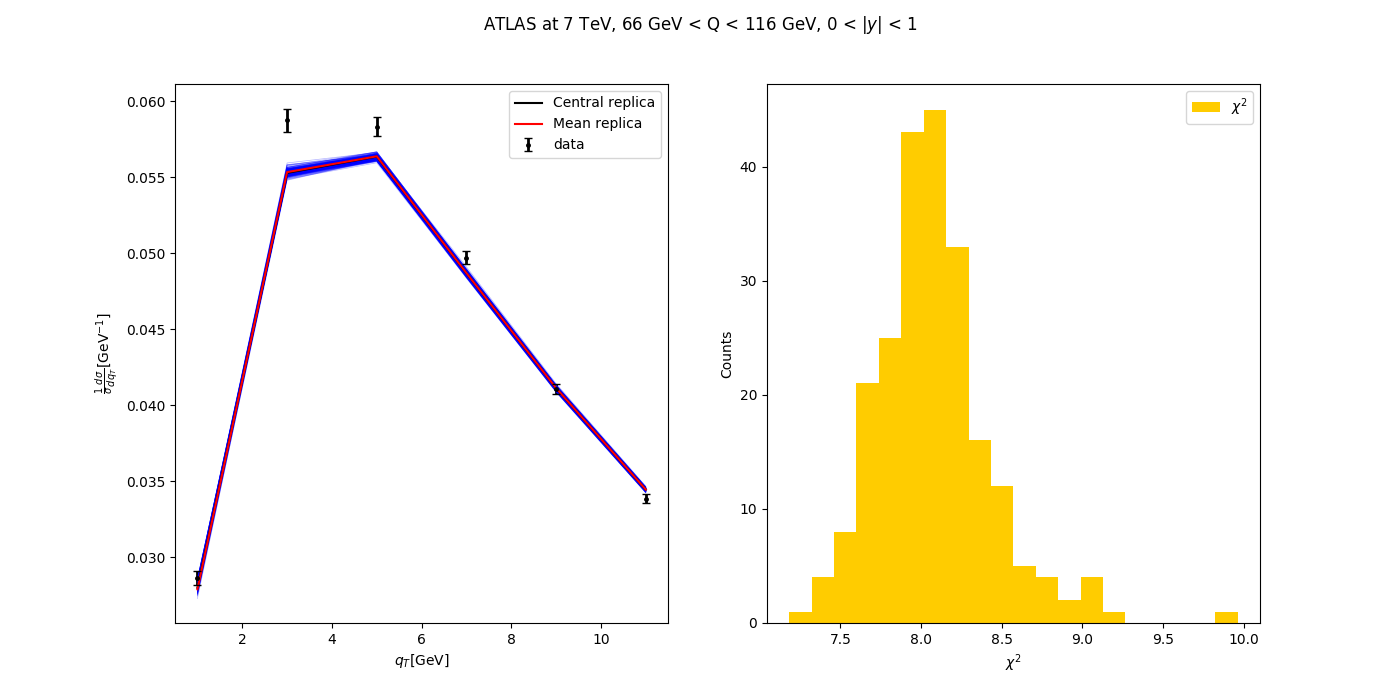
\includegraphics{pngplots/ATLAS_7TeV_y_0_1.png}
\caption{ATLAS\_7TeV\_y\_0\_1 data-theory comparison}
\end{figure}

\begin{figure}
\centering
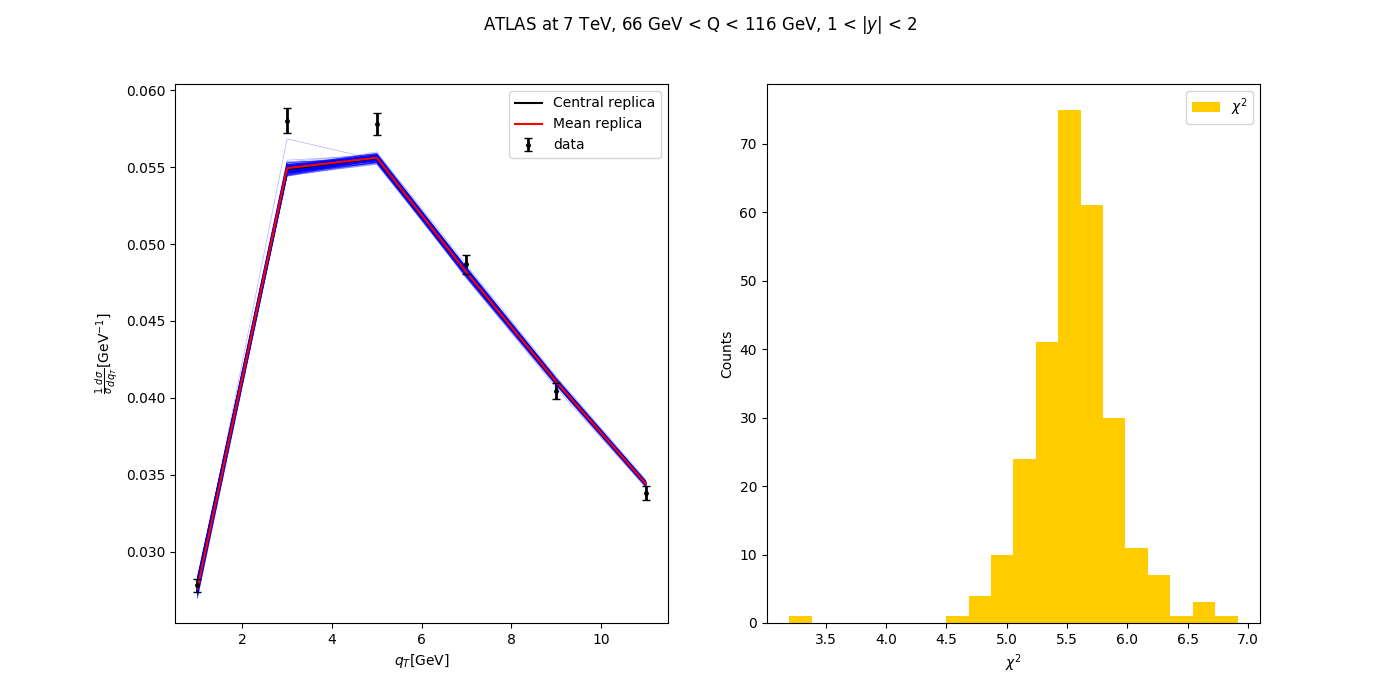
\includegraphics{pngplots/ATLAS_7TeV_y_1_2.png}
\caption{ATLAS\_7TeV\_y\_1\_2 data-theory comparison}
\end{figure}

\begin{figure}
\centering
\includegraphics{pngplots/ATLAS_7TeV_y_2_2.4.png}
\caption{ATLAS\_7TeV\_y\_2\_2.4 data-theory comparison}
\end{figure}

\begin{figure}
\centering
\includegraphics{pngplots/ATLAS_8TeV_y_0_0.4.png}
\caption{ATLAS\_8TeV\_y\_0\_0.4 data-theory comparison}
\end{figure}

\begin{figure}
\centering
\includegraphics{pngplots/ATLAS_8TeV_y_0.4_0.8.png}
\caption{ATLAS\_8TeV\_y\_0.4\_0.8 data-theory comparison}
\end{figure}

\begin{figure}
\centering
\includegraphics{pngplots/ATLAS_8TeV_y_0.8_1.2.png}
\caption{ATLAS\_8TeV\_y\_0.8\_1.2 data-theory comparison}
\end{figure}

\begin{figure}
\centering
\includegraphics{pngplots/ATLAS_8TeV_y_1.2_1.6.png}
\caption{ATLAS\_8TeV\_y\_1.2\_1.6 data-theory comparison}
\end{figure}

\begin{figure}
\centering
\includegraphics{pngplots/ATLAS_8TeV_y_1.6_2.png}
\caption{ATLAS\_8TeV\_y\_1.6\_2 data-theory comparison}
\end{figure}

\begin{figure}
\centering
\includegraphics{pngplots/ATLAS_8TeV_y_2_2.4.png}
\caption{ATLAS\_8TeV\_y\_2\_2.4 data-theory comparison}
\end{figure}

\begin{figure}
\centering
\includegraphics{pngplots/ATLAS_8TeV_Q_46_66.png}
\caption{ATLAS\_8TeV\_Q\_46\_66 data-theory comparison}
\end{figure}

\begin{figure}
\centering
\includegraphics{pngplots/ATLAS_8TeV_Q_116_150.png}
\caption{ATLAS\_8TeV\_Q\_116\_150 data-theory comparison}
\end{figure}

\end{document}
